% !TeX program = xelatex
% EvoGenesis 论文（中文草稿，数学建模体）。
%
% 章节结构与本仓库 paper/报告-骨架.md「§1 章节结构与文件映射」一一对应。
% 写作主轴（赛题补充说明）：为什么要改 -> 改了什么 -> 实际结果如何 -> 具有什么价值与意义。
% 正文只写模型与方法；开发过程、仓库路径、票据号、状态词不进正文（见骨架 §2）。
\documentclass[11pt,a4paper]{ctexart}
% 导言区：中文草稿版（xelatex + ctexart）。
% 换英文/换会议时，只需替换本文件的「字体与版式」两段为会议官方 sty，见 README。
\usepackage{amsmath,amssymb}
\usepackage{tikz}
\usetikzlibrary{arrows.meta,positioning,calc}
\usepackage{algorithm}
\usepackage{algpseudocode}
\usepackage{graphicx}
\usepackage{booktabs}
\usepackage{array}
\usepackage{siunitx}
\usepackage{xcolor}
\usepackage{tabularx}
\usepackage{threeparttable}
\usepackage{float}
\usepackage{subcaption}
\usepackage{multirow}
\usepackage[numbers,sort&compress]{natbib}
\usepackage{gbt7714}
\usepackage[hidelinks]{hyperref}
\usepackage{url}

\graphicspath{{figs/}}          % 论文用图统一放 paper/latex/figs/（自包含，不依赖 results/）

% --- 版式（中文草稿）---。换会议时整段替换为官方 sty 的版式约定。
\usepackage[a4paper,margin=2.5cm]{geometry}
\ctexset{
  section/format = \Large\bfseries,
  subsection/format = \large\bfseries,
}
\linespread{1.25}

% 断行兜底：中英混排的长串（路径、指标名）不可断，靠拉伸量吸收余量，避免溢出边界
\setlength{\emergencystretch}{3em}
\sloppy
\tolerance=3000
\hbadness=10000

% 统一占位标记：未写的内容必须显式可见，禁止用编造内容填充
\newcommand{\todo}[1]{\textcolor{red}{[TODO: #1]}}


\title{\bfseries 发育式编码的神经网络架构：从基因调控网络到可演化、可模仿学习的斑马鱼智能体}
\author{李辰钊 \and 池伟豪}
\date{\today}

\begin{document}
\maketitle
\tableofcontents

\begin{abstract}
\todo{写完正文后回来压成 200 字以内；须含四个数：结构规模、训练前后对照、与 baseline 的差、}
\todo{一条可复现的结论。禁止在没跑完实验前写具体数字。}
\end{abstract}

\noindent\textbf{关键词：} 神经架构设计；发育式编码；基因调控网络；演化计算；行为克隆

\section{问题重述}\label{sec:problem}

\subsection{问题背景}

当代深度网络的能力主要由两件事决定：\textbf{人工指定的架构}与大数据上的参数拟合。
生物智能体则不同：它的网络拓扑由一段紧凑的基因组经\textbf{发育过程}生成，
而个体一生中由经验造成的突触改变\textbf{不会写回基因组}，
即所谓 genomic bottleneck：遗传信息必须先于网络结构，后天学习不得遗传
\citep{bib1_zador2019,bib2_barabasi2023,bib3_shuvaev2024}。

围绕这一差别，已有三条相关研究线索。神经演化（neuroevolution）在网络结构或权重空间上直接搜索
\citep{bib5_miikkulainen2025}；其生成式路线把可演化对象从权重扩展到结构或生成规则，
如 NEAT 以历史标记交叉直接演化拓扑 \citep{bib222_stanley2002}，
HyperNEAT 由一个 CPPN 按几何坐标查询生成连接权重 \citep{bib223_stanley2009}，
增强版 ES-HyperNEAT 进一步让位置与密度可演化 \citep{bib124_risi2012}。
发育式编码路线已证明紧凑基因组可以编码先天能力 \citep{bib1_zador2019,bib3_shuvaev2024}，
并以发育先验生成权重矩阵 \citep{bib2_barabasi2023}，
或用简单随机发育的生成模型重建小脑连接组 \citep{bib4_richter2025}。
神经架构搜索（NAS）则在离散的层、算子、连接空间上搜索
\citep{bib224_elsken2019}，或把该空间连续松弛为混合算子权重以便梯度优化 \citep{bib225_liu2019}。
上述工作的评价场景多为静态基准；近年用发育程序长出网络的近作
\citep{bib226_najarro2023} 仍以静态机器学习基准评价。

本文的切入点是：把\textbf{可演化的对象上移一层}，搜索空间是生成网络结构的基因组，
网络结构是发育算子的产物，并按 genomic bottleneck 的要求把当代学习限制为
不接受遗传的权重扰动；评价放进\textbf{闭环生态仿真}，使结构与行为通过感知—动作回路耦合，
从而可以在同一平台上分别测量「结构多样性」「结构—行为联系」「当代可塑性的代价」。

\subsection{问题提出}

本文围绕以下两个问题建立模型并求解：

\begin{enumerate}
  \item 若让\textbf{网络架构本身}由基因组、发育、连接组逐级生成，
        能否得到既\textbf{可用}（可完成任务）又\textbf{多样}（不同基因型给出系统性不同的结构）的网络？
  \item 若把学习严格限制为\textbf{当代权重的有界扰动}且\textbf{不接受其遗传}，
        要为此付出什么代价？这一限制究竟是负担，还是塑造了可演化的结构？
\end{enumerate}

据此构建 \textsc{EvoGenesis} 作为可复现的计算实验平台，主要工作包括四部分：
(i) 提出「基因组—发育—连接组—行为」的三层生成式架构模型（\S\ref{sec:model}）；
(ii) 构建二维闭环生态仿真环境，把行为评价落到觅食、避敌、能量与生长（\S\ref{sec:solution}）；
(iii) 建立与三类主流网络（MLP、GRU、稀疏循环网络）在同参数量级下的对照，
      回答「改之前与改之后」的差异（\S\ref{sec:solution}）；
(iv) 量化基因型到架构的可辨识性、环境依赖性与误差范围，并给出模型评价与推广（\S\ref{sec:validation}、\S\ref{sec:evaluation}）。

\textbf{重点与范围。}本文的重心是建模机制：从基因型到连接组的生成链、当代学习与遗传边界、
闭环生态评价，均给出完整的数学形式与可运行实现（\S\ref{sec:model}），
并在此基础上给出已完成的对照与检验结果（\S\ref{sec:solution}、\S\ref{sec:validation}）；
训练类实验按计算预算分批推进。配套前端展示与工程仓库已搭建完成，
代码、演示与复现说明见 \url{https://github.com/54cwh/mathHackathon} 。

\section{问题分析}\label{sec:analysis}

\subsection{总体思路}

本文把「网络架构由基因组经发育生成」抽象为一条\emph{确定性推进的生成管线}，
并用一条\emph{遗传边界}把当代学习与代际遗传分开。管线为

\begin{equation}\label{eq:pipeline}
G\;\text{ 经 } D_{\Theta} \text{ 得 }\; (A,Z,\tau,W^{(0)},M)
\;\text{ 再由 DanioNet 得 }\; \mathcal{T}
\;\text{ 经 }\mathcal{F}\text{ 评 }\; F
\;\text{ 经 }\mathcal{R}\text{ 产生 }\; \mathcal{P}_{t+1},
\end{equation}

其中 $G$ 为人工二倍体基因组，$D_\Theta$ 为发育算子（基因调控网络、细胞命运、发育式连接生成），
$A,Z,\tau,W^{(0)},M$ 分别为连接矩阵、细胞身份、时间常数、发育初始权重与活跃神经元掩码，
$\mathcal{T}$ 为个体在环境中的行为轨迹，$F$ 为适应度，$\mathcal R$ 为代际更新。
\textbf{当代学习}发生在轨迹之前：$W^{*}=L(W^{(0)},A,Z,\tau,\mathcal{D},K)$，
$L$ 只更新连接权重的幅度，且产生的增量 $\Delta W$ 不进入下一代。

采用这条管线的理由是\emph{受控对照}：被检验的命题链是
「不同 DNA 故不同架构，故不同行为，故不同环境不同演化结局」，
而只有仿真能做到只改一个碱基、其余全部相同。
本模型不使用任何外部数据集训练，全部数据由受控仿真生成，
每个数字都能由同一配置与同一随机种子确定性重放。

\subsection{技术路线}

建模数据流如图~\ref{fig:pipeline}，分生成链、同源分支、代际闭环三段。

\textbf{生成链。}自随机种子到行为轨迹是一条确定性生成链：配置与随机种子经种子管理派生基因组 $G$，
$G$ 经发育算子 $D_{\Theta}$ 生成连接组 $(A,Z,\tau,W^{(0)},M)$，
再由 DanioNet 在连续二维生态仿真（$20$\,Hz $\times$ $600$ 步每回合）中驱动得到行为轨迹 $\mathcal{T}$。
随机种子是唯一的随机入口，调控读出 $q(G)$ 是基因型影响连接组的唯一通路；
因此单碱基扰动、以及同源基因组在不同随机种子下的实现，都是可测量的结构变异来源。

\textbf{同源分支。}仿真之后，同一次运行产生三路共用编号、可相互对齐的数据：
专家轨迹（规则控制器逐步记录观测与动作，用于行为克隆）、
事件日志（用于实验指标）、帧快照（用于实时演示）。
磁盘日志是演示推送的超集，推送的每条记录都能在日志中找到。

\textbf{代际闭环与遗传边界。}适应度 $F$ 经选择与漂变产生下一代基因组，回到生成链顶端；
后代不携带任何当代学习增量。图中红虚线框标出\textbf{遗传边界}：行为克隆只改变权重的幅度，
其增量 $\Delta W$ 不进入繁殖通路，后代只继承基因组并从发育重新开始（\S\ref{method:bc}）。

\begin{figure}[H]
  \centering
  \resizebox{\linewidth}{!}{%
  \begin{tikzpicture}[
    font=\scriptsize,
    box/.style={draw, rounded corners, align=center, minimum height=0.72cm, inner sep=3pt},
    gen/.style={box, fill=green!8, minimum width=3.6cm},
    sim/.style={box, fill=orange!14, minimum width=15cm, minimum height=0.9cm},
    br/.style={box, fill=violet!8, minimum width=3.0cm},
    evo/.style={box, fill=blue!6, minimum width=2.6cm},
    bound/.style={box, draw=red, dashed, fill=red!4, minimum width=3.6cm},
    ar/.style={-{Latex}, thick},
    gar/.style={-{Latex}, thick, green!55!black},
  ]
    \node[gen] (seed) at (0,10.0) {配置与随机种子};
    \node[gen] (genome) at (0,9.0) {基因组（碱基串与调控基序）};
    \node[gen] (dev) at (0,8.0) {发育（调控网络 / 连接生成）};
    \node[gen] (conn) at (0,7.0) {连接组（DanioNet，至多 48 节点）};
    \node[sim] (arena) at (0,5.9) {生态仿真（$20$\,Hz $\times$ $600$ 步 / 回合）};

    \node[evo] (fit) at (-6.6,4.5) {适应度 $F$};
    \node[evo] (sel) at (-6.6,3.5) {选择 / 漂变};
    \node[evo] (next) at (-6.6,2.5) {下一代基因组};

    \node[br] (t1) at (-2.6,4.5) {专家轨迹};
    \node[br] (t2) at (-2.6,3.5) {行为克隆};
    \node[bound] (dw) at (-2.6,2.5) {权重增量 $\Delta W$\\（当代，不遗传）};

    \node[br] (l1) at (1.4,4.5) {事件日志};
    \node[br] (l2) at (1.4,3.5) {实验指标};

    \node[br] (s1) at (5.4,4.5) {帧快照};
    \node[br] (s2) at (5.4,3.5) {实时演示};

    \draw[ar] (seed) -- (genome);
    \draw[ar] (genome) -- (dev);
    \draw[ar] (dev) -- (conn);
    \draw[ar] (conn) -- (arena);
    \draw[ar] (arena.south) -- ++(0,-0.45) -| (t1.north);
    \draw[ar] (arena.south) -- ++(0,-0.45) -| (l1.north);
    \draw[ar] (arena.south) -- ++(0,-0.45) -| (s1.north);
    \draw[ar] (arena.west) -- ++(-0.9,0) |- (fit.west);
    \draw[ar] (t1) -- (t2);
    \draw[ar] (t2) -- (dw);
    \draw[ar] (l1) -- (l2);
    \draw[ar] (s1) -- (s2);
    \draw[ar] (fit) -- (sel);
    \draw[ar] (sel) -- (next);

    \draw[gar] (next.west) -- ++(-1.0,0) |- (genome.west);

    \node[align=left, font=\scriptsize, text=red] at (2.2,1.7)
      {遗传边界：$\Delta W$ 只作用于当代，\emph{不进入繁殖通路}；\\后代只继承基因组并从发育重新开始。};
  \end{tikzpicture}}
  \caption{整体数据流（技术路线图）。}
  \label{fig:pipeline}
\end{figure}

\subsection{关键问题与待检验命题}\label{sec:rq}

由两个中心问题拆出五个待检验命题（H1--H5），构成本文的分析主线：

\begin{itemize}
  \item \textbf{H1}：不同基因组在相同随机种子控制下产生\textbf{系统性}的连接组差异。
  \item \textbf{H2}：连接组与神经元动力学的差异导致行为差异。
  \item \textbf{H3}：异质时间常数 $\tau_i$ 形成与同质 $\tau$ 不同的\textbf{性能—效率权衡}。
  \item \textbf{H4}：空间布线代价改变网络的局部性、稀疏性与有效边效率。
  \item \textbf{H5}：$F=F(G,E)$，\textbf{不存在对所有环境都占优的基因型}。
\end{itemize}

对应的量化判据（阈值属独立标定任务，不在本文主张内）：
H1 用组内图距离并以重连零模型为基线 \citep{bib20_hartle2020}；
H2 用 Mantel 检验 \citep{bib21_smouse1986}；
H3 用性能—效率 Pareto 前沿 \citep{bib23_deb2002}；
H4 以平均连接距离度量局部性，并与图论效率区分命名 \citep{bib22_latora2001}；
H5 用 reaction norm 与 AMMI 检验基因型与环境的秩反转
\citep{bib24_via1985,bib25_malosetti2013}。

\textbf{统计能力有限}：正式实验的独立随机种子数为 $3$，
此时 $3$ 对 $3$ 标签置换检验的双侧最小 $p\approx0.10$，
不足以支持逐命题的置换检验。H1 采用组内口径、H2 采用 Mantel 检验，
二者均不依赖 $3$ 对 $3$ 置换；其余结论以效应量与跨种子波动并列报告
（见 \S\ref{sec:solution} 与 \S\ref{sec:validation}）。

\subsection{设计要点与创新}\label{sec:innovation}

本文的竞争力在建模设计。整个模型围绕三个设计要点展开，它们互相约束、缺一不可：

\begin{enumerate}
  \item \textbf{把可演化的对象上移一层。}主流做法在网络结构或权重空间上直接搜索，
        本文让被搜索的对象是\textbf{生成结构的基因组}，网络结构是发育算子的产物。
        由此，同源基因组与不同随机种子、单碱基扰动都成为可测量的结构变异来源，
        结构变异与基因变异可分（\S\ref{method:genome}、\S\ref{method:dev}）。
  \item \textbf{用一条遗传边界把先天与后天分开。}当代学习只改变量幅度，
        $\Delta W$ 不进入繁殖通路，后代只继承基因组并从发育重新开始。
        这把 genomic bottleneck 由一句主张变成可对照的实验条件：
        当代可塑性承担了多少、发育结构承担了多少，可以分别测量（\S\ref{method:bc}）。
  \item \textbf{在闭环生态里同时度量可用与多样。}评价不走静态基准，
        而走感知—动作回路与环境耦合的连续二维生态仿真，
        使「结构多样性」与「行为可用性」在同一条链上被观测（\S\ref{method:net}、\S\ref{sec:solution}）。
\end{enumerate}

表~\ref{tab:related} 概括本文设计与三类相关工作的差别。
三个要点的组织方式决定了后文的顺序：\S\ref{sec:model} 给出每个子模型的数学形式与设计依据，
\S\ref{sec:solution} 给出可复核的结果证据。

\begin{table}[H]
  \centering
  \caption{本文设计与相关工作的对照。}
  \label{tab:related}
  \footnotesize
  \setlength{\tabcolsep}{2pt}
  \begin{threeparttable}
  \resizebox{\linewidth}{!}{\begin{tabular}{@{}p{0.14\linewidth}p{0.2\linewidth}p{0.2\linewidth}p{0.2\linewidth}p{0.22\linewidth}@{}}
    \toprule
    维度 & 神经演化 & 神经架构搜索 & 发育式编码 & 本文 \\
    \midrule
    可演化对象 & 网络结构或权重 & 架构（层、算子、连接） & 基因组到权重的映射 & 基因组（结构是发育产物） \\
    生成规则 & 直接变异与交叉 & 离散搜索或连续松弛 & 发育先验生成权重 & 调控网络与连接生成组成的发育过程 \\
    遗传边界 & 未显式区分 & 训练所得权重即解 & 侧重先天编码能力 & 显式：当代增量 $\Delta W$ 不遗传 \\
    评价场景 & 多为静态基准 & 静态基准的验证精度 & 静态基准或连接组重建 & 连续二维闭环生态仿真 \\
    \bottomrule
  \end{tabular}}
  \begin{tablenotes}\footnotesize\raggedright
    \item 代表文献：神经演化 \citep{bib5_miikkulainen2025,bib222_stanley2002,bib223_stanley2009}；
          神经架构搜索 \citep{bib224_elsken2019,bib225_liu2019}；
          发育式编码 \citep{bib1_zador2019,bib2_barabasi2023,bib4_richter2025}。
  \end{tablenotes}
  \end{threeparttable}
\end{table}


\section{模型假设}\label{sec:assumptions}

本节集中列出建模所用的假设。每条给出依据与失效后果；后文不再重复声明。

\begin{enumerate}
  \item \textbf{基因组先于网络结构。} 个体由二倍体基因组 $G$（离散碱基串与调控基序）描述，
        碱基不直接编码权重，只经基因调控网络影响细胞命运，网络结构是发育算子的产物。
        依据：genomic bottleneck \citep{bib1_zador2019,bib3_shuvaev2024}。
        失效后果：若碱基直接编码权重，发育层的解释力消失，结构变异与基因变异将不再可分。

  \item \textbf{二倍体结构与等位基因效应的通路单一化。} 个体含两对同源染色体，
        等位基因效应只经调控读出 $q(G)$ 传给基因调控网络。
        依据：孟德尔式结构分离需要二倍体与独立分配；通路单一化使单碱基与结构变化可归因。
        失效后果：位点表达量若另行进入发育，则变异来源混杂，单碱基扰动的效应不可辨识。

  \item \textbf{同源链聚合取加性平均，调控读出用失配等权的简化相似度。}
        依据：加性是定量遗传的标准基线 \citep{bib138_fisher1918}，简化相似度可解释、可编辑。
        失效后果：加性会抹平完全显性；简化式丢位置权重，须以 PWM 与逐基序取最大作对照（\S\ref{sec:validation}）。

  \item \textbf{发育过程有限且同分布。} 初始前体细胞均分到六个功能域，每个前体至多分裂一次，
        神经元数 $N\in[24,48]$；位置取域内均匀随机。
        依据：发育式连接生成需要「同一机制、不同随机实现」的可控变异性。
        失效后果：若分裂次数无上界，结构规模不受控，对照实验的固定容量假设失效。

  \item \textbf{连接概率由类型兼容、空间代价与表达相似度三项决定。}
        依据：线性距离项等价于指数距离规则，有连接组学支撑 \citep{bib125_ercseyravasz2013}；
        随机放置已足以复现特异功能连接 \citep{bib123_hill2012}。
        失效后果：空间代价系数有量纲、绑定归一化发育方域，若改用文献的毫米口径则不可比。

  \item \textbf{突触符号由突触前类型决定（Dale 约束），时间常数逐神经元异质。}
        依据：抑制性前神经元自抑制等定性符号模式 \citep{bib14_dorkenwald2024}；
        异质整合时间与 NMDA、GABA$_B$ 及数百毫秒决策整合同量级。
        失效后果：时间常数的语义是网络级整合常数，区别于单神经元膜常数的量级。

  \item \textbf{神经元动力学取离散漏积分发放形式，非线性取双曲正切。}
        依据：$\tau\ge1$ 时状态是自身与有界非线性的凸组合，零输入下状态有界。
        失效后果：若 $\tau<1$ 则 $1/\tau>1$ 放大状态，有界性不再成立。

  \item \textbf{感官增益、输入权重偏置与神经元偏置按细胞类型固定，不参与学习。}
        依据：保持发育输出契约 $(A,Z,\tau,W^{(0)},M)$ 冻结，感官通路仍经细胞类型与基因型挂钩。
        失效后果：若这些量可学习，则「结构由发育生成」的主张被稀释，参数量对照口径改变。

  \item \textbf{当代学习只改连接权重幅度，支撑与符号在训练期冻结。}
        依据：genomic bottleneck 要求后天学习不得遗传；结构只能在代际经基因组变异改变。
        失效后果：结构在当代不可改变，这是本文要测量的代价之一（对应 H1、H3）。

  \item \textbf{适应度取四项行为指标代内归一后的加权和，选择用二元锦标赛。}
        依据：四项覆盖生存、觅食、避敌、能量四个生态维度；锦标赛对适应度的平移与线性变换不变
        \citep{bib136_blickle1996,bib137_eiben2015}，而比例选择强度与适应度尺度不可分离 \citep{bib135_goldberg1991}。
        失效后果：$F$ 只是代内相对分数，不可跨代、跨环境直接比较；权重属设计选择，须做敏感性分析。

  \item \textbf{环境为连续二维闭环，边界反射，回合长度固定。}
        依据：反射边界确定性、不消耗随机数，跨种子对照才成立；固定长度使分母固定、跨回合可比。
        失效后果：幸存个体在全灭后仍空转至回合上限，这些步不携带行为信息（代价被接受）。

  \item \textbf{突变率 $\mu=0.001$ 每碱基每配子属计算抽象参数。}
        依据：与数字演化惯例同量级（Avida 默认约 $0.0075$）。
        失效后果：它比脊椎动物真实种系碱基替换率高约 $10^{5}$ 倍，不可作生物学参数解读。
\end{enumerate}

\section{符号说明}\label{sec:notation}

本文符号与 \S\ref{sec:analysis} 式~\eqref{eq:pipeline} 一致，主要符号如表~\ref{tab:notation}。

\begin{table}[H]
\centering
\caption{主要符号与含义。}
\label{tab:notation}
\footnotesize
\setlength{\tabcolsep}{4pt}
\resizebox{\linewidth}{!}{\begin{tabular}{@{}lll@{}}
  \toprule
  符号 & 含义 & 单位 / 取值 \\
  \midrule
  $G$ & 二倍体基因组（碱基串与调控基序） & 512\,bp \\
  $q(G)$ & 基因组经调控网络的读出 & $[0,1]^{8}$ \\
  $\mathbf g_i$ & 第 $i$ 个细胞的调控网络状态 & $\mathbb{R}^{8}$ \\
  $M_k$ & 第 $k$ 个调控基序 & 6\,bp，共 8 个 \\
  $D_{\Theta}$ & 发育算子（调控网络、细胞命运、连接生成） & --- \\
  $N$ & 活跃神经元数 & 整数，$[24,48]$ \\
  $\mathbf p_i$ & 第 $i$ 个细胞在发育方域内的位置 & 归一化单位 \\
  $A$ & 连接邻接矩阵（二值） & $N\times N$ \\
  $Z$ & 细胞身份（六类功能域的后验） & 概率向量 \\
  $\tau_i$ & 第 $i$ 个神经元的整合时间常数 & $[1,10]$ \\
  $W^{(0)}$ & 发育初始连接权重 & 实矩阵 \\
  $M$ & 活跃神经元掩码 & 二值向量 \\
  $h_i^{t}$ & 第 $i$ 个神经元在 $t$ 步的状态 & $(-1,1)$ \\
  $x_t$ & 第 $t$ 步的观测向量 & $[0,1]^{12}$ \\
  $U_i,\,m_i,\,b_i$ & 感官增益、输入权重、偏置（按细胞类型固定） & 实数 \\
  $\phi$ & 神经元非线性 & $\tanh$ \\
  $\omega_t,\,v_t$ & 第 $t$ 步的转向与推进动作 & $\omega\in[-1,1],\ v\in[0,1]$ \\
  $\Theta$ & 当代学习优化的参数张量 & 与 $W^{(0)}$ 同形 \\
  $W$ & 实际连接权重 & $W=A\odot(\operatorname{sign}(W^{(0)})\odot\mathrm{softplus}(\Theta))$ \\
  $\Delta W$ & 当代学习产生的权重增量（不遗传） & 实矩阵 \\
  $L$ & 当代学习算子 & --- \\
  $F$ & 适应度 & 代内 $[0,1]$ \\
  $S,P,E_{\mathrm{esc}},Q$ & 生存、捕食、逃脱、净能量四分量 & $[0,1]$ \\
  $E_t$ & 能量 & $[0,E_{\max}]$，$E_{\max}=1$ \\
  $H_t$ & 饥饿 & $[0,1]$，$H_t=1-E_t/E_{\max}$ \\
  $\lambda,\,\gamma$ & 空间布线代价、表达相似度系数 & $\lambda=2.0$，$\gamma=1.0$ \\
  $\rho$ & 调控网络状态更新率 & $0.35$ \\
  $\mu$ & 每碱基每配子的突变率 & $0.001$ \\
  $T$ & 回合长度 & $600$ 步（$20$\,Hz，$30$\,s） \\
  \bottomrule
\end{tabular}}
\end{table}

\section{模型的建立}\label{sec:model}\label{sec:method}

本节按数据流\textbf{自上而下}组织：先说明基因型与调控网络（\S\ref{method:genome}），
再依次给出发育（\S\ref{method:dev}）、连接组（\S\ref{method:net}）、
当代学习（\S\ref{method:bc}）与演化闭环（\S\ref{method:evo}）。
每个设计选择均给出依据与代价；符号沿用 \S\ref{sec:notation}，管线沿用式~\eqref{eq:pipeline}。
连接组的生成机制如图~\ref{fig:mechanism}。

\begin{figure}[H]
  \centering
  \resizebox{\linewidth}{!}{%
  \begin{tikzpicture}[
    font=\scriptsize,
    gen/.style={draw, rounded corners, align=center, minimum height=0.85cm, inner sep=4pt, fill=green!8},
    proc/.style={draw, rounded corners, align=center, minimum height=0.85cm, inner sep=4pt, fill=orange!12},
    ar/.style={-{Latex}, thick},
    bound/.style={draw, dashed, red, rounded corners, align=center, fill=red!4, inner sep=4pt},
  ]
    \node[gen, minimum width=3.0cm] (g) at (0,0) {基因组\\（碱基串与调控基序）};
    \node[proc, minimum width=3.0cm] (grn) at (3.8,0) {调控网络\\读出 $q(G)$};
    \node[proc, minimum width=3.0cm] (fate) at (7.6,0) {细胞命运\\（六类功能域）};
    \node[proc, minimum width=3.6cm] (wire) at (11.7,0) {连接概率\\（类型兼容、空间代价、表达相似度）};
    \node[gen, minimum width=3.6cm] (conn) at (16.0,0) {连接组\\$(A,Z,\tau,W^{(0)},M)$};
    \node[bound, minimum width=5.2cm] (bc) at (16.0,-1.7) {当代学习：增量 $\Delta W$（不遗传）};
    \draw[ar] (g) -- (grn);
    \draw[ar] (grn) -- (fate);
    \draw[ar] (fate) -- (wire);
    \draw[ar] (wire) -- (conn);
    \draw[ar] (conn) -- (bc);
  \end{tikzpicture}}
  \caption{连接组的生成机制。}
  \label{fig:mechanism}
\end{figure}

\subsection{基因型与调控网络}\label{method:genome}

\textbf{设计选择}：基因组是\textbf{离散碱基串与调控基序目录}，碱基不直接编码权重，
表达量经\textbf{调控网络}（GRN）给出细胞命运。

\paragraph{基因组布局。}个体为二倍体：2 对同源染色体，每条单倍体染色体 $128$\,bp，
故配子 $256$\,bp、二倍体全基因组 $2\times2\times128=\mathbf{512}$\,bp，
字母表 $\{$A,C,G,T$\}$。第 0 代种群不植入基序，4 条链共 512 个碱基在字母表上
\textbf{均匀独立同分布}抽取。调控基序目录为 8 条、每条 $6$\,bp，
在实验随机种子下\textbf{一次性抽样后固定}，跨个体、跨代不变。

\paragraph{读出 $q(G)$。}单链基序相似度取简化式
$a(M_k,s)=1-d_H(M_k,s)/|M_k|$（$d_H$ 为 Hamming 距离），整条序列取
$q_k(S)=\mathrm{TopKMean}_{s\subset S}\,a(M_k,s)$（窗口 $6$\,bp、步长 1、$K=3$），
两条同源链按\textbf{加性平均}合并：

\begin{equation}\label{method:eq-qg}
q(G)=\tfrac12\bigl(q^{(h1)}+q^{(h2)}\bigr)\in[0,1]^8 ,
\qquad
\mathbf g_i^{r+1}=(1-\rho)\,\mathbf g_i^{r}
+\rho\,\sigma\!\bigl(W_g\mathbf g_i^{r}+B\,q(G)+P\mathbf p_i+\mathbf b\bigr).
\end{equation}

右式为离散调控网络：8 维状态，默认 12 步、$\rho=0.35$、$\sigma$ 为 sigmoid、
初态 $\mathbf g_i^{0}=\mathbf 0$；$W_g\in\mathbb R^{8\times8}$ 取 Xavier uniform 后重标定
至谱半径 $0.9$。窗口在\textbf{各染色体内}滑动、不跨染色体边界。

\paragraph{依据与代价。}二倍体与独立分配是孟德尔式结构分离的前提；
把等位基因效应压到 $q(G)$ 一条通路，才能让单碱基与结构的变化可归因。
代价是位点表达量不进入发育，只作为报告层的阈值读出；
加性平均会\textbf{抹平完全显性}，故把逐基序取最大（完全显性投影）留作消融对照；
简化相似度\textbf{丢失位置权重}，须配 PWM 对照；
基序目录固定后，跨实验比较必须共享同一种子家族，否则 $q(G)$ 的坐标系不同、不可直接比较。

\subsection{发育：从调控网络到连接组}\label{method:dev}

\textbf{设计选择}：区别于由基因组直接指定连接，网络结构由\textbf{发育过程}从调控网络终态生成。

\textbf{依据}：这是 genomic bottleneck 的机制主张，遗传信息先于网络结构
\citep{bib1_zador2019,bib3_shuvaev2024}；以发育先验生成权重矩阵
\citep{bib2_barabasi2023} 与用简单随机发育生成模型重建小脑连接组
\citep{bib4_richter2025} 已有先例。把可演化的对象上移一层，也使
同源基因组与不同随机种子的组合、以及单碱基扰动，都成为可测量的结构变异来源。

\paragraph{发育流程。}初始 24 个前体细胞，均分到 6 个发育域
（sensory / prey / threat / integrator\_memory / inhibitory / motor，每域 4 个），
位置取\textbf{域分块均匀随机}（归一化发育单位方域划为 $3\times2$ 个 block，按域行优先填入）。
每个前体\textbf{至多分裂一次}，
$p_i^{\mathrm{divide}}=\sigma(\mathbf w_d^\top\mathbf g_i^{12}+b_d)$，
分裂扰动加到位置与调控网络终态上，故 $24\le N\le 48$。
细胞身份由 $\mathbf l_i=U\mathbf g_i+\mathbf c_{domain(i)}$、
$\mathbf z_i=\mathrm{softmax}(\mathbf l_i)$、$type_i=\arg\max_k z_{ik}$ 给出。
连接概率为

\begin{equation}\label{method:eq-lij}
P(A_{ij}=1)=\sigma\bigl(\underbrace{\mathbf z_i^\top C\mathbf z_j}_{\text{type 兼容}}
\underbrace{-\lambda d_{ij}}_{\text{空间代价}}
+\underbrace{\gamma R(\mathbf g_i,\mathbf g_j)}_{\text{表达相似度}}
+b_A\bigr),\qquad d_{ij}=\lVert \mathbf p_i-\mathbf p_j\rVert_2,
\end{equation}

不允许自环；$b_A$ 用二分反解使\emph{期望}非对角密度 $=0.15$。
初始权重幅度 $\lvert w^{(0)}_{ij}\rvert=\mathrm{softplus}\bigl(\mathbf u^\top[\mathbf g_i;\mathbf g_j;\mathbf z_i;\mathbf z_j]+b_w\bigr)$，
符号由\textbf{突触前}类型决定（Dale 式约束）：

\begin{equation}\label{method:eq-dale}
\operatorname{sign}(w_{ij})=
\begin{cases}
-1, & type_i=\text{Inhibitory},\\
+1, & \text{otherwise};
\end{cases}
\qquad
\tau_i=\tau_{\min}+(\tau_{\max}-\tau_{\min})\,\sigma(\mathbf a^\top\mathbf g_i+b_\tau)\in[1,10].
\end{equation}

发育产物为 $(A,Z,\tau,W^{(0)},M)$。其中 $A$ 为二值邻接、$Z$ 为细胞身份、
$\tau$ 为时间常数、$W^{(0)}$ 为初始有效权重、$M$ 为活跃神经元掩码。

\paragraph{依据与代价。}六类细胞类型是\textbf{功能抽象}，划分参照斑马鱼感觉运动回路与
全脑连接组组织 \citep{bib6_petrucco2023,bib7_dunn2016,bib14_dorkenwald2024}，
不对应特定真实细胞类型；真实细胞类型远超六类 \citep{bib84_kunst2019}，
且 $\arg\max$ 是离散化理想化，真实命运是连续谱 \citep{bib75_moris2016}。
连接概率含空间布线代价 $-\lambda d_{ij}$（$\lambda=2.0$，在归一化单位方域上取值），
logit 中的线性距离项等价于指数距离规则 $P\propto e^{-\lambda d}$，有连接组学支撑
\citep{bib125_ercseyravasz2013}，随机放置已足以复现特异功能连接 \citep{bib123_hill2012}；
代价是 $\lambda$ \textbf{有量纲}、绑定本项目的归一化方域口径，不能照搬文献的毫米口径值，
故 $\lambda=0$ 须作消融对照（对应 H4）。
表达相似度项取逐分量标准化后的\textbf{双线性}形式，$\gamma=1.0$ 固定、零额外参数，按弱偏置使用
\citep{bib111_qiao2024,bib112_kovacs2020,bib119_sanes2020}；
单用表达相似度预测连线的证据仅 AUC$\approx0.64$，且有反 Hebbian 的反例 \citep{bib121_hayashi2022}，
故须报告 $\gamma=0$ 消融与 $\{0.5,1,2\}$ 敏感性搜索。
类型兼容先验 $C$ 取\textbf{人工固定矩阵}，给出抑制性前神经元自抑制、
sensory 不互相兴奋这类定性符号模式 \citep{bib14_dorkenwald2024}；
其数值\textbf{无外部依据}，属项目设计选择，只作定性参照。

\paragraph{良构判据。}三类判据缺一不可：(i) \textbf{发育}，每类命运至少 1 个，
motor 至少各有 1 个左右输出神经元；(ii) \textbf{功能}，存在 sensory 到 motor 的有向路径；
(iii) \textbf{动力学}，零输入下从零态跑 50 步无 NaN/Inf、$\lvert h_i^t\rvert<1$
（该式是 $h_i^t$ 与 $\tanh(\cdot)$ 的凸组合，由零初态归纳即得，属模型的数学性质）、
尾部 10 步平均饱和比例 $<0.9$、谱半径 $\rho(W^{(0)})<1$；后两条为工程判据。

良构通过率如图~\ref{fig:viability}。四个面板依次为累计通过率与 Wilson 区间、各判据失败次数、
谱半径分布与阈值、随机 $q$ 与管线 $q(G)$ 的口径对照。正式配置下 $1000$ 次随机 $q$ 全部通过
（Wilson $[99.6\%,100.0\%]$），八项判据零次触发：判据 (ii) 与 (iv) 及命运缺失项由设计约定保证，
恒真而不贡献区分力。故发育算子的作用是构造可行结构，筛选压力归代际适应度 $F$。

\begin{figure}[H]
  \centering
  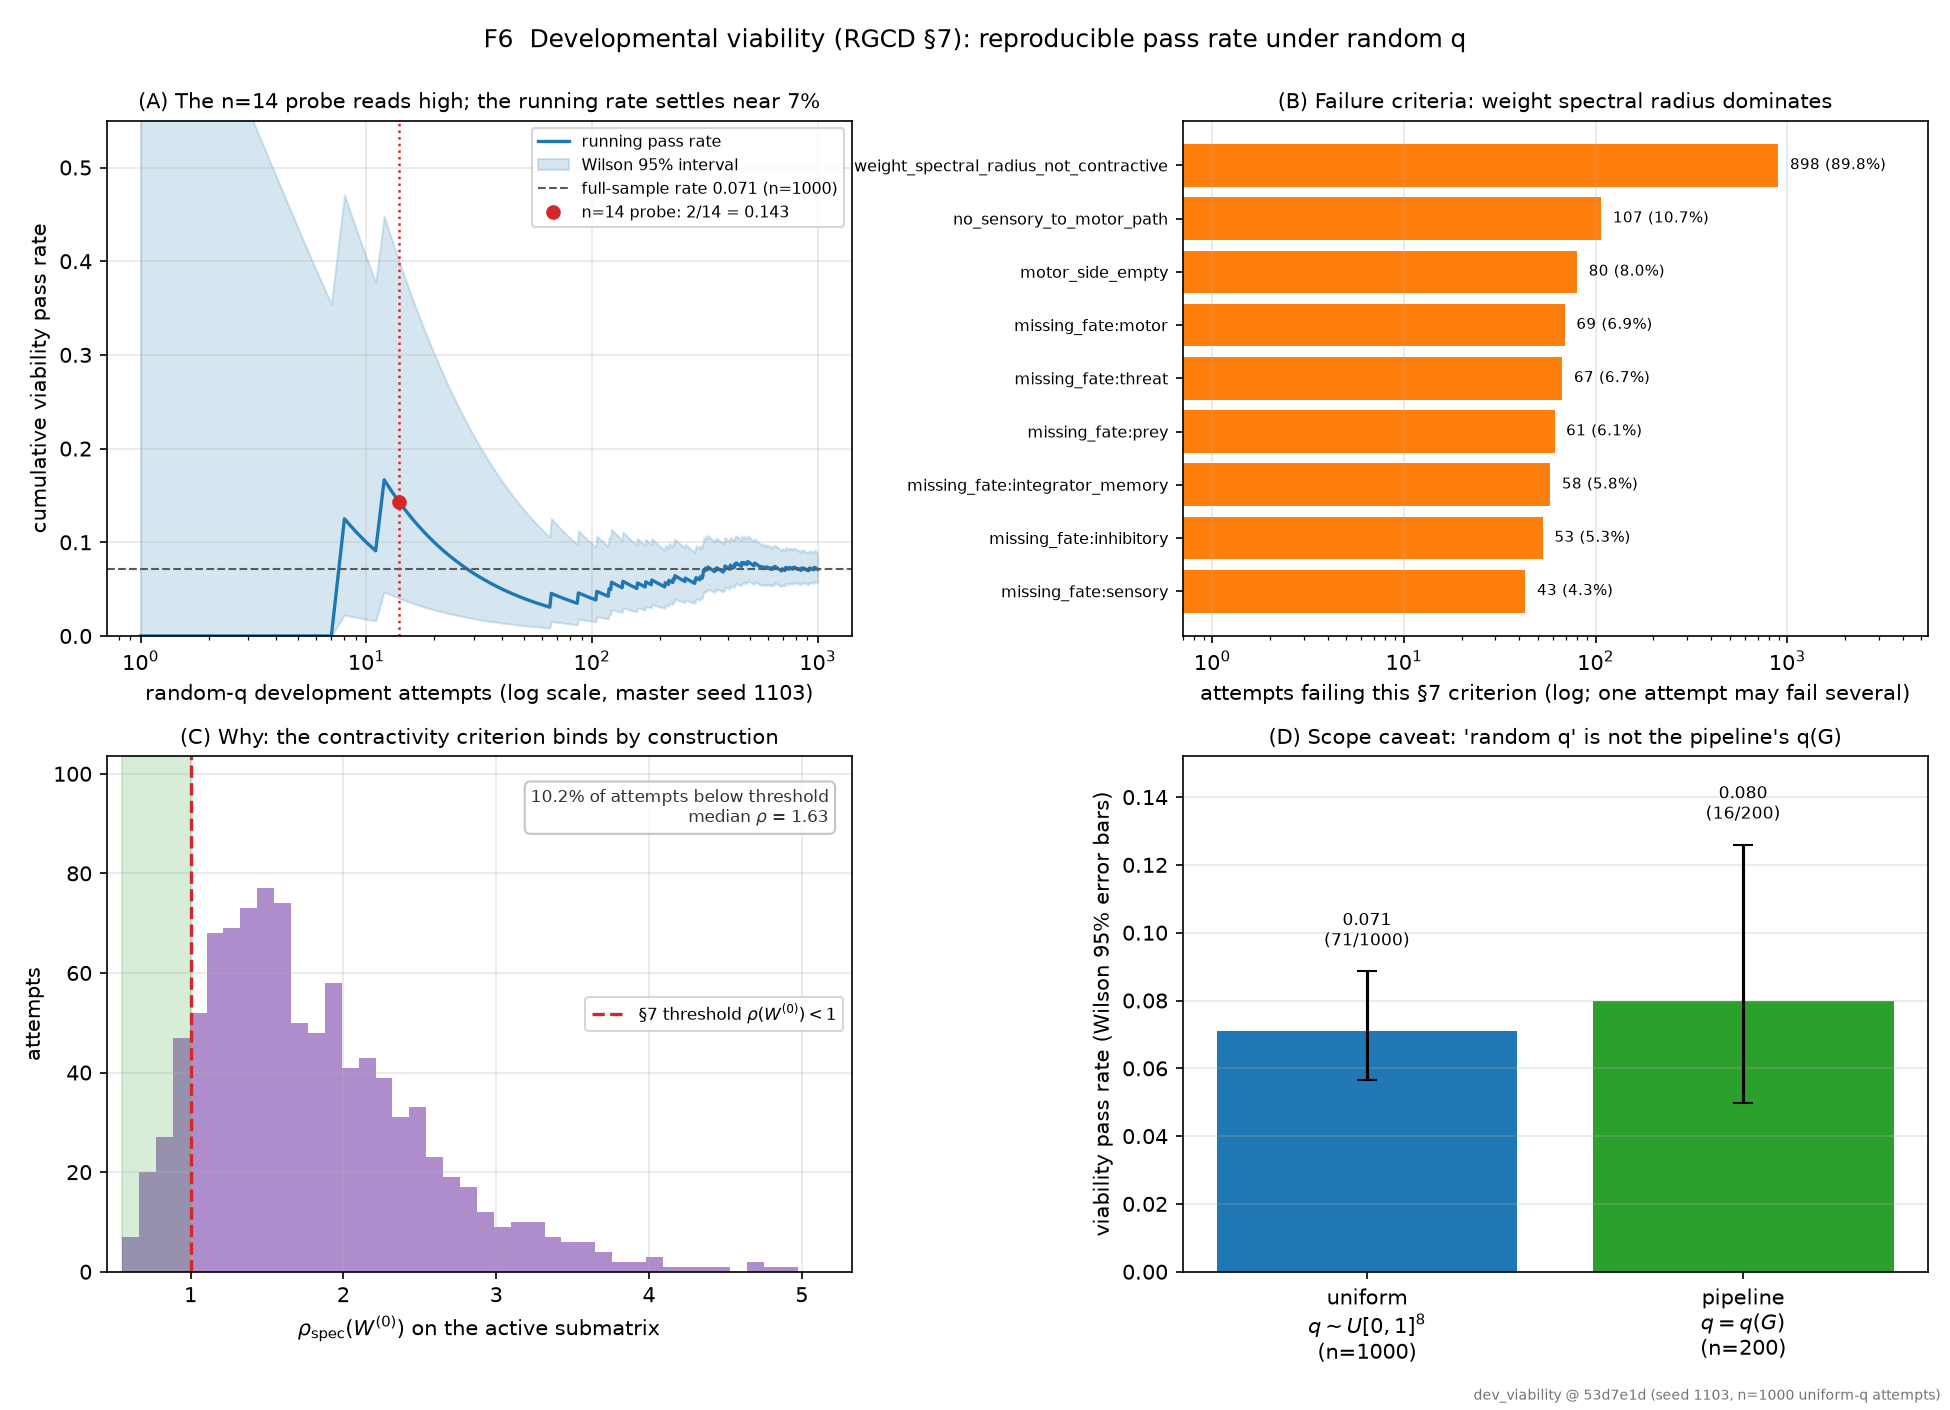
\includegraphics[width=0.96\linewidth]{fig_viability}
  \caption{发育良构通过率。}
  \label{fig:viability}
\end{figure}

\subsection{网络结构：DanioNet 与 48 节点}\label{method:net}

\textbf{设计选择}：把发育产物当作一个\textbf{漏积分发放（firing-rate）离散网络}来跑，
状态维数按容量上界 $48$ 分配张量，再用掩码界定真正活跃的部分。

\paragraph{48 节点的含义。}$48$ 是\textbf{容量上界}，逐基因型的实际规模由发育决定。
发育产出的活跃神经元数 $N$ 落在 $[24,48]$。在 3 个正式种子 $\times$ 14 个体共 42 个基因型上实测：
$N$ 中位 $37.0$（27--43），支撑连接中位 $192.5$ 条（105--289），
密度中位 $0.149$（由目标密度经 $b_A$ 二分反解保证）。
网络张量在批内补零到 48，由神经元掩码 $M$ 与邻接掩码 $A$ 共同界定参与计算的神经元，
非活跃神经元的行与列恒 0。

\paragraph{可训练参数量。}被优化的 $\Theta$ 张量形状为 $48\times48=2304$，
但\textbf{有效可训练的只有支撑之内的那些边}，实测中位 $192.5$ 条（个体间 105--289），
即 $\mathcal O(10^2)$ 量级，其余位置被掩码屏蔽、梯度恒 0。
与基线做参数量同一数量级对照时，以此为准（\S\ref{sec:solution}）。

\paragraph{动力学。}网络为

\begin{equation}\label{method:eq-dyn}
h_i^{t+1}=\Bigl(1-\tfrac{1}{\tau_i}\Bigr)h_i^{t}
+\tfrac{1}{\tau_i}\,\phi\Bigl(\sum_j A_{ij}w_{ij}h_j^{t}+U_i x_t+m_i H_t+b_i\Bigr),
\end{equation}

默认 $\phi=\tanh$；$\tau\ge1$ 是前提（$\tau<1$ 被拒，因 $1/\tau>1$ 会放大）。
$U_i,m_i,b_i$ 按\textbf{细胞类型}取固定先验、不学习，使发育输出契约 $(A,Z,\tau,W^{(0)},M)$ 保持冻结，
感官增益仍经细胞类型与基因型挂钩。

\paragraph{动作。}取\textbf{均值池化}：$\omega_t=\tanh(y_\omega)$、$v_t=\sigma(y_v)$，其中

\begin{equation}\label{method:eq-action}
y_\omega=\overline{h}_{M_L}-\overline{h}_{M_R},\qquad
y_v=\overline{h}_{M_{\mathrm{motor}}},\qquad
\omega_t\in[-1,1],\ v_t\in[0,1],
\end{equation}

$M_L,M_R$ 为左右 motor 池、$M_{\mathrm{motor}}$ 为全 motor 池。左池主导得 $\omega>0$。

\paragraph{输入。}12 维观测由网络侧冻结：语义、顺序、值域 $[0,1]$、dtype \texttt{float32}；
左右两个通道各自的猎物种群强度、天敌强度、障碍强度（6 维），
最近可见猎物与天敌的相对体型（2 维），天敌视角扩张率（1 维），
上一步推进（1 维），能量与饥饿（2 维，互补且和恒为 1）。其中饥饿即式~\eqref{method:eq-dyn} 的 $H_t=x_t[11]$。

\paragraph{依据与代价。}动力学取漏积分发放的离散形式、时间常数逐神经元异质 $\tau_i\in[1,10]$：
在 20\,Hz（$\Delta t=50$\,ms）下，$\tau_i$ 步等效 $50$--$500$\,ms 的网络级整合时间常数，
与 NMDA / GABA$_B$ 及数百毫秒决策整合同量级，异质性本身是 H3 的处理变量；
作为\textbf{单神经元膜时间常数}该量偏大（皮层约 20\,ms），其语义是网络级整合。
动作取均值池化，对池大小不变、零新参数，代价是丢弃池内分布信息。
左右 motor 按发育坐标中位数二分，保证两池非空、直接满足良构判据。
输入取 12 维\textbf{结构化感知向量}，捕食与威胁分通道对应斑马鱼视觉的捕食与威胁回避通路
\citep{bib8_trivedi2013,bib58_temizer2015,bib60_semmelhack2014}，
饥饿与能量对应内部状态对决策的调制 \citep{bib9_filosa2016,bib10_zaupa2024}；
结构化编码本身是建模假设，区别于从像素学得。

图~\ref{fig:connectome} 中左为 $48\times48$ 的 $W^0$（含填充）与活跃的 $N\times N$ 块，
中为按细胞类型分块的权重符号结构，右为 $N$ 与支撑边数的群体分布。

\begin{figure}[H]
  \centering
  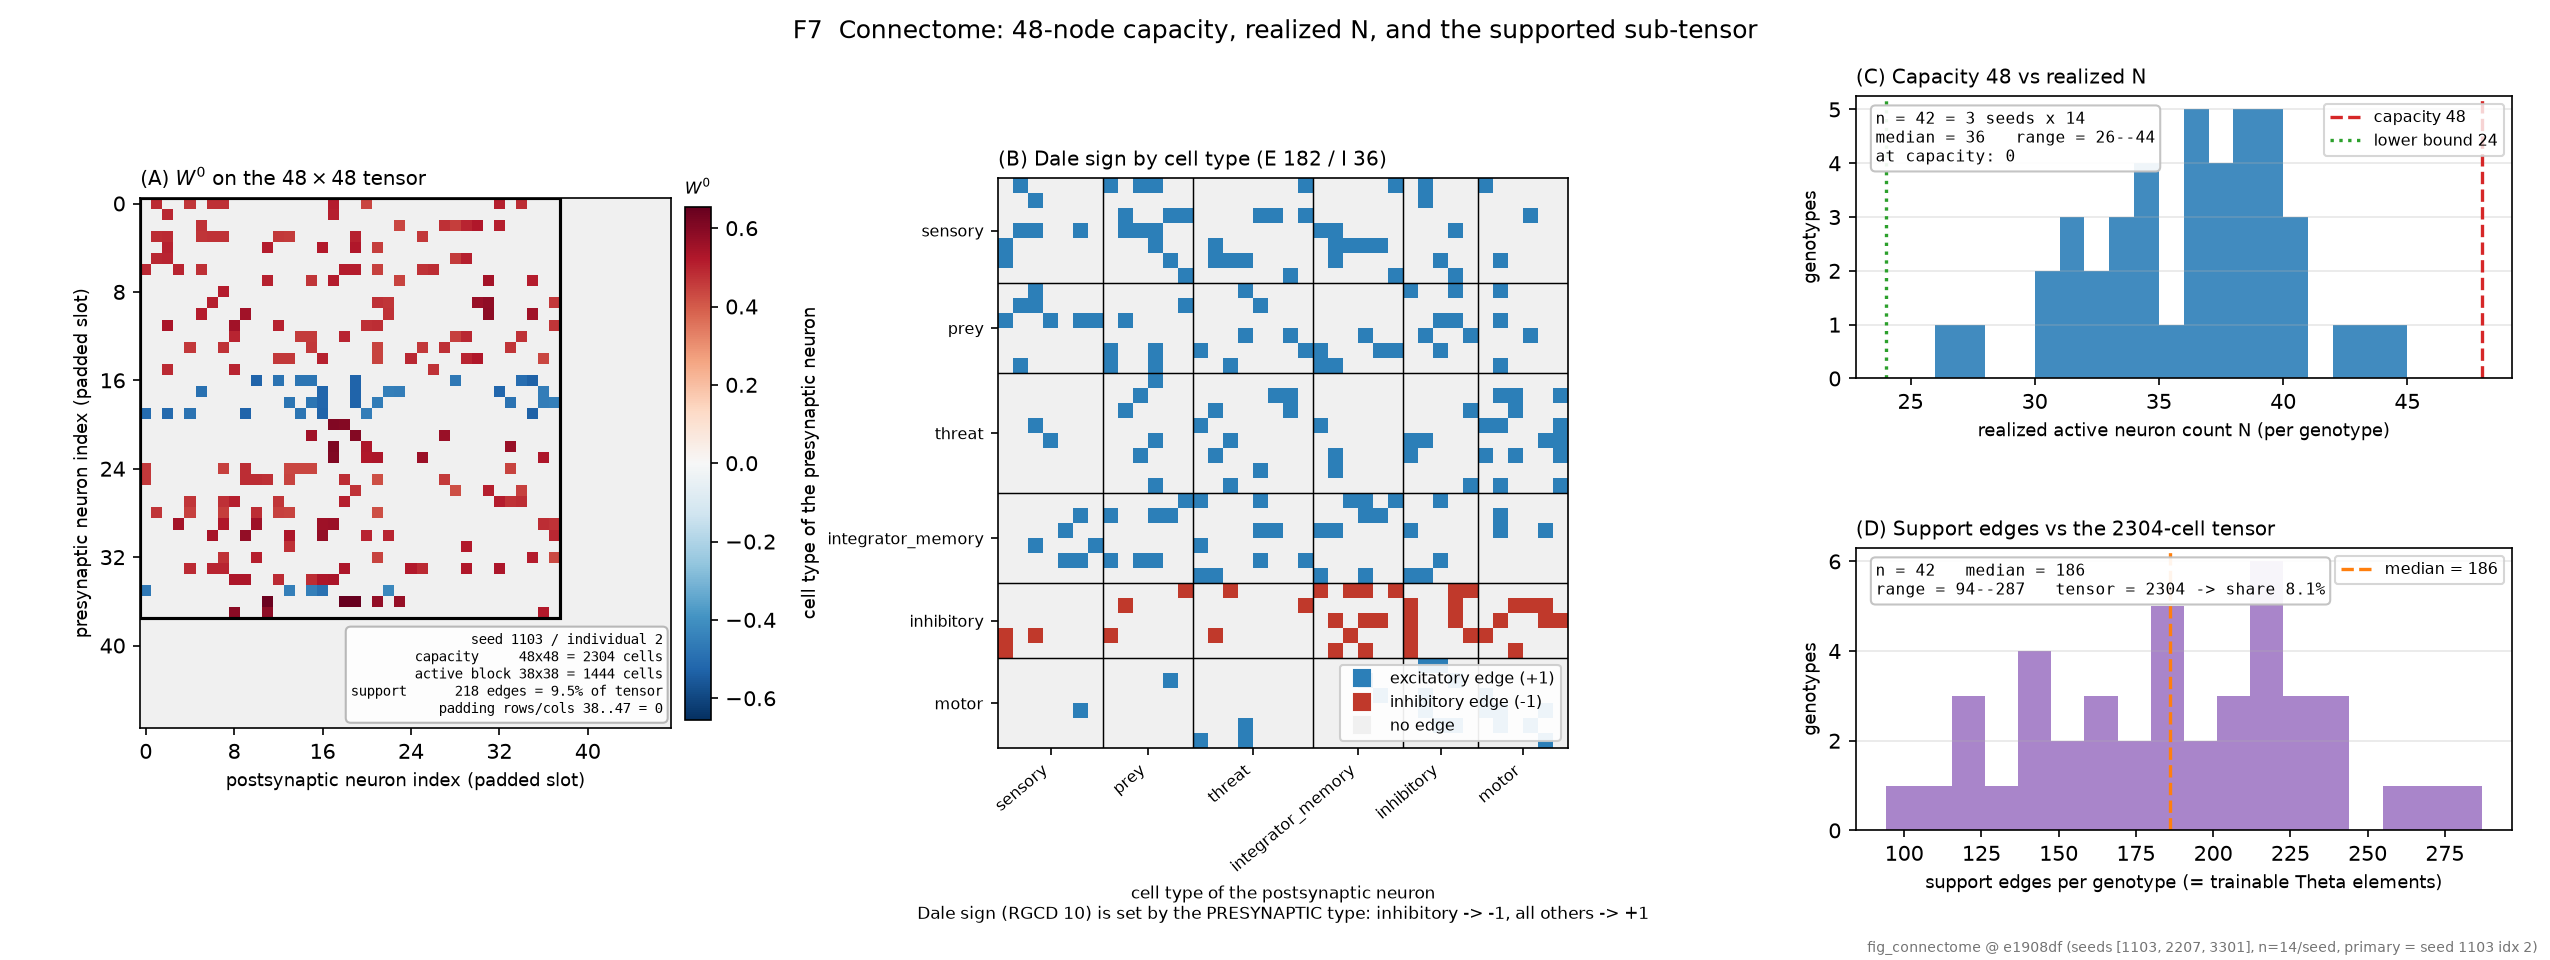
\includegraphics[width=\linewidth]{fig_connectome}
  \caption{连接矩阵与结构统计。}
  \label{fig:connectome}
\end{figure}

\subsection{当代学习：行为克隆}\label{method:bc}

\textbf{设计选择}：唯一的学习环节是\textbf{行为克隆}，且它只改\textbf{当代}权重、
\textbf{不进入繁殖通路}。遗传边界为

\begin{equation}\label{method:eq-boundary}
\text{DNA 经调控网络到发育，得 } W^{(0)}
\text{ 再经当代学习，得 } \Delta W \quad(\text{不遗传}),
\end{equation}

后代只继承 DNA，并从发育重新开始。训练对象被参数化为

\begin{equation}\label{method:eq-wtheta}
W=A\odot\Bigl(\operatorname{sign}(W^{(0)})\odot\mathrm{softplus}(\Theta)\Bigr),
\qquad
\Theta^{0}=\mathrm{softplus}^{-1}\bigl(\lvert W^{(0)}\rvert\bigr)
\ \Longrightarrow\ \Delta W=0,
\end{equation}

被优化的是 $\Theta$（与 $W^{(0)}$ 同形），支撑 $A$ 与
$\operatorname{sign}(W^{(0)})$ 在训练期\textbf{冻结}：不新增连接、不翻转符号，
$\Delta W=W-W^{(0)}$ 是导出量。

\paragraph{数据。}教师是\textbf{透明的规则控制器} ExpertPolicy
（视野内追踪最近猎物、按威胁与障碍转向），可解释。它驱动鱼、逐步记录
$(\text{observation},\text{expert\_action})$ 样本；每条回合只记录 1 条受控鱼
（其余个体照常存在以提供真实感知上下文），标准预算 200 条回合对应约 $1.2\times10^{5}$ 个步样本。

\paragraph{训练。}$\Delta W$ 是\textbf{逐个体}的：DNA 不同，故网络不同，
故每个当代个体各自训练自己的网络（同一份专家数据、各自的 $\Theta$）。
因零初态时 $W h^{0}=0$、单步梯度恒 0，故按回合顺序\textbf{整段展开 BPTT}：
每次更新抽 64 条回合为一 batch，每条自零初态前向满 600 步，
先对回合内逐步损失取均值、再对 batch 取均值后整段回传。预算 20 次更新、Adam、学习率 $10^{-3}$。
损失按目标尺度归一化后求加权 MSE：

\begin{equation}\label{method:eq-bcloss}
\lambda_i=\frac{1}{\max(\sigma_i,\ 0.05R_i)^{2}},\quad i\in\{\omega,v\},
\qquad
\mathcal L=\lambda_\omega\,\mathrm{MSE}(\hat\omega,\omega^{*})
+\lambda_v\,\mathrm{MSE}(\hat v,v^{*}),
\end{equation}

其中 $\sigma_i$ 为训练集上第 $i$ 维动作的总体标准差、$R_\omega=2,R_v=1$ 为取值跨度，
权重整体缩放至 $\lambda_\omega+\lambda_v=2$，等价于对各维目标 z-score 后等权，
故 $\lambda$ \textbf{无量纲、非自由超参}，只改损失尺度，不改式~\eqref{method:eq-action} 的有界映射。

\paragraph{依据与代价。}$\Delta W$ 不遗传：这是 genomic bottleneck 的核心主张
\citep{bib1_zador2019,bib3_shuvaev2024}；评估阶段必须由 DanioNet 驱动，
否则 DNA 与学习都不影响行为、适应度失去意义。代价是学习收益\textbf{每代都要重新付出}、无法积累，
且结构在当代\textbf{不可改变}，这是本文要测量的代价之一（对应 H1、H3）。

\subsection{演化闭环：适应度、选择与漂变}\label{method:evo}

\textbf{设计选择}：闭环为 $F$ 经选择与漂变得到下一代 $G'$，
其中选择算子取\textbf{二元锦标赛}、繁殖规模\textbf{恒定}。

\paragraph{适应度。}用四项原始行为指标的加权和

\begin{equation}\label{method:eq-fitness}
F=0.35\,S+0.25\,P+0.20\,E_{\mathrm{esc}}+0.20\,Q ,
\end{equation}

$S$ 为生存、$P$ 为捕食、$E_{\mathrm{esc}}$ 为逃脱、$Q$ 为净能量积累率。
四项各自在\textbf{代内良构个体}上做 min-max 归一到 $[0,1]$
（某分量当代 $\max=\min$ 时该分量置 0），故 $F$ 是\textbf{代内相对分数}。

\paragraph{遗传算子与漂变。}每对染色体以 0.5 概率发生一次单点交叉（切点取自内部断点），
随后随机选一条进入配子；配子上施加 SNP 替换突变，
$\mu=0.001$ 每碱基每配子（256\,bp 单倍体对应每个配子期望 0.256 个新突变）。
种群规模 $48$，随机配子与随机后代抽样\textbf{自然产生}遗传漂变，不额外引入漂变参数。

\paragraph{依据与代价。}适应度取四项代内归一后的加权和，覆盖生存、觅食、避敌、能量四个生态维度，
使各分量与量纲无关、权重之和为 1；代价是 $F$ \textbf{只是代内相对分数}，
不可跨代、跨环境比较，跨代与跨环境一律改用原始指标，且四位权重须做敏感性分析。
二元锦标赛尺度无关（对适应度的平移与线性变换不变，且在期望适应度分布上等价于最大线性排名
\citep{bib136_blickle1996,bib137_eiben2015}），而比例选择的强度与适应度尺度不可分离
\citep{bib135_goldberg1991}；代价是尺度无关以\textbf{有放回}抽样为前提。
亲本池\textbf{只含良构个体}，non-viable 排除。
每代恒产 $48$ 个后代、世代不重叠，使漂变强度跨代可比。
SNP 替换率与数字演化惯例同量级（Avida 默认约 $0.0075$），
比脊椎动物真实种系碱基替换率高约 $10^{5}$ 倍，故\textbf{不可作生物学参数解读}。

\paragraph{闭环回到起点。}下一代的基因组重新进入式~\eqref{eq:pipeline} 的顶端，
且\textbf{不携带任何 $\Delta W$}：结构从发育重新生成，当代权重从 $\Delta W=0$ 重新开始。
这条回路与式~\eqref{method:eq-boundary} 的边界共同定义本文的实验对象。
生成-演化主循环如算法~\ref{alg:loop} 所示。

\begin{algorithm}[H]
\caption{生成-演化主循环}\label{alg:loop}
\begin{algorithmic}[1]
\Require 配置与 master seed；种群规模 $N_p=48$；代数 $T$
\Ensure 逐代记录：基因组与结构统计、行为指标与适应度
\State 由 master seed 派生各命名空间子种子
\State 初始化第 $0$ 代种群（512\,bp 随机基因组）
\For{$t \gets 0$ \textbf{to} $T-1$}
  \State 每个基因组经发育算子生成 $(A,Z,\tau,W^{(0)},M)$，并做良构判定
  \State 每个良构个体在生态仿真中跑一回合，得行为轨迹
  \State 由轨迹计算四分量，代内归一得适应度 $F$
  \If{启用当代学习}
    \State 以专家轨迹做行为克隆，更新当代权重 $\Delta W$（不遗传）
  \EndIf
  \State 二元锦标赛选择亲本，经交叉与突变得下一代基因组
\EndFor
\State \Return 逐代记录
\end{algorithmic}
\end{algorithm}

\section{模型的求解与结果分析}\label{sec:solution}\label{sec:results}\label{sec:experiment}\label{sec:baselines}

本章给出环境的设置（\S\ref{sec:exp-env}）、与三类基线网络的对比（\S\ref{sec:baselines-ours}）、
环境对照（\S\ref{sec:exp-env-groups}）、基因型到架构的可辨识性（\S\ref{sec:pen}），
以及学习前后对照与典型案例。尚未取得落盘结果的项在正文中标为待补。
呈现以图为主、表为辅，且「改之前与改之后」保持同图同轴可比。

\subsection{实验设置与参考基线}\label{sec:exp-env}

\textsc{Danio Arena} 是一个\textbf{连续二维、闭环}的觅食—避敌环境：被测对象是
DanioNet 个体网络，其行为由感知—动作回路与环境耦合产生。

\paragraph{世界与时钟。}世界为 $100\times60$ 世界单位的连续二维平面，
更新频率 $20$\,Hz（$\Delta t=0.05$\,s），一个标准回合为 $30$\,s $=600$ 步。
默认对象为 12 条鱼、24 只猎物、3 只天敌、6 个障碍。\textbf{两种种群规模不混用}：
本文基线与环境对照用 12 鱼，世代演化用 48 个个体的种群。

\paragraph{边界。}取镜面反射边界：越界分量取反射，朝向按墙法线镜面反射。
该策略确定性、不消耗随机数，故不会扰动同一随机种子下的随机流，跨种子对照才成立。

\paragraph{生理机制。}能量按
$E_{t+1}=\mathrm{clip}(E_t-C_{\text{base}}-C_{\text{move}}v_t^2-C_{\text{pen}}p_t
+R_{\text{food}}f(\text{size}_{\text{prey}})\mathbb{1}_{\text{cap}},0,E_{\max})$
演化（$p_t$ 为本步障碍穿透深度，$\mathbb{1}_{\text{cap}}$ 为本步是否捕获的指示函数），
饥饿 $H_t=1-E_t/E_{\max}$，能量归零即死亡；
吃到猎物后按面积守恒带损耗生长
$\text{size}\leftarrow\min(\text{size}_{\max},\sqrt{\text{size}^2+g\,\text{size}_{\text{prey}}^2})$，
故体型增大带来可捕食更大猎物的收益，同时付出代谢成本上升与转向灵活性下降
（$\omega_{\text{eff}}=\omega/[1+k_{\text{turn}}(\text{size}-1)]$）的代价。
生长增益 $g$ 的取值区间参照开源游戏实现 \citep{bib215_testn.d.}，属工程对照，不作学术依据；
$30$\,s 内真实鱼的质量变化仅 $\sim10^{-5}$ 量级，故局内可见的生长是游戏化抽象，须放到跨回合与世代尺度讨论。

\paragraph{捕食与再生。}捕食需\textbf{同时}满足三条：距离 $d<r_{\text{capture}}$、
体型门 $\text{size}_{\text{hunter}}\ge\kappa\,\text{size}_{\text{target}}$、
且目标位于猎人朝向的前向锥内（$\theta_{\text{cone}}=120^\circ$ 为总锥角）。
其中 $\kappa=1.25$ 属设计选择：未找到斑马鱼直接的最大可吞猎物与体长上限，
替代物种的 $20$--$27\%$ 体长度量的是猎物体高，不可倒数为 $\kappa$ \citep{bib221_mihalitsis2017}。
前向锥 $120^\circ$ 与限时追击 $80$ 步同属设计选择，机制对照来自开源游戏实现
\citep{bib217_tghbrkn.d.,bib218_monkwarriorn.d.}，不是经验证的生物学量。
猎物走开放可再生：存活猎物数低于设定时按固定间隔补 1 只。
鱼每步遍历猎物时命中第一个进入捕获半径的猎物即处理并退出，
故每鱼每步\textbf{至多}产生一条捕获判定。回合结束只由步数决定，一律跑满 600 步；
个体死亡只冻结该个体，空种群不提前结束，故生存率以固定分母计算。
生态仿真的关键设定列于表~\ref{tab:arena-config}。

\begin{table}[H]
  \centering
  \caption{生态仿真的关键设定。}
  \label{tab:arena-config}
  \footnotesize
\setlength{\tabcolsep}{1pt}
  \resizebox{\linewidth}{!}{\begin{tabular}{@{}lll@{}}
    \toprule
    设定 & 值 & 说明 \\
    \midrule
    世界 $W\times H$ & $100\times60$ wu & 世界单位 \\
    更新频率 / $\Delta t$ & $20$ Hz / $0.05$ s & 时钟步长 \\
    标准回合 & $30$ s $=600$ 步 & 固定长度 \\
    规模（基线） & 12 鱼 / 24 猎物 / 3 天敌 / 6 障碍 & 与种群规模分离 \\
    规模（演化） & 48 个体 & 世代演化 \\
    边界 & 镜面反射 & 确定性、不耗随机数 \\
    感知半径 / 视野 & $18.0$ wu / $220^\circ$ & 受限感知 \\
    捕获半径 $r_{\text{capture}}$ & $4.61$ wu & 几何判定 \\
    体型门 $\kappa$ & $1.25$ & 设计选择 \\
    前向锥 $\theta_{\text{cone}}$ & $120^\circ$（总锥角） & 设计选择 \\
    能量系数 & $E_{\max}=1.0$, $C_{\text{base}}=0.0008$, & \\
     & $C_{\text{move}}=0.0015$, $R_{\text{food}}=0.12$ & \\
    生长上限 / 增益 & $\text{size}_{\max}=2.5$, $g=0.2$ & $g$ 为设计选择 \\
    逃脱存活窗口 & 20 步（$=1$ s） & 设计选择 \\
    限时追击 & 80 步 & 设计选择 \\
    \bottomrule
  \end{tabular}}
\end{table}

\paragraph{感知。}个体不拥有全图信息，只有左右两条视觉通道、有限感知半径与有限视野；
网络每步接收一个 12 维观测向量，其值域与顺序由网络侧冻结（\S\ref{method:net}）。

\paragraph{度量口径。}本节的口径是三处最容易被误读的地方，引用对应数字时必须同时带上。

\textbf{（一）三个都叫捕获率的量，数值差约 7 倍。}
\begin{enumerate}
  \item \textbf{绝对速率}：个体单位时间捕食数 $\overline{(\text{captures}_i/\text{episode\_steps})}$，无偏、可跨环境直接比较；
  \item \textbf{接触转化率}：个体层面 $\overline{(\text{captures}_i/\text{encounters}_i)}$，即追近的猎里有多少吃到；
  \item \textbf{汇总比值}：$\sum_i\text{captures}_i/\sum_i\text{encounters}_i$，按遭遇次数加权。
\end{enumerate}
实测（基线，3 种子 $\times$ 12 鱼）：接触转化率的个体均值为 $0.5407$，
而汇总比值为 $55/722=0.0762$，两者相差 $7.1$ 倍。原因是前者为个体比值的等权平均
（把一个只遇到 1 次猎物却恰好捕获的个体与一个遇到 200 次的个体同等看待），后者按遭遇次数加权。
正文与图表所报的比值一律指\textbf{接触转化率的个体均值}。

\textbf{（二）接触转化率的分母语义。}其定义为
\begin{equation}\label{eq:prey-capture}
  \text{prey\_capture}_i \;=\; \frac{\text{captures}_i}{\max(\text{encounters}_i,\,1)} .
\end{equation}
分母 $\text{encounters}$ 是\textbf{尺寸门之前的纯距离接触计数}：鱼每步遇到首个
$d<r_{\text{capture}}$ 的猎物即自增并退出，故它计的是进入捕获半径的次数，与尺寸门和
前向锥都无关。分母取 $\max(\cdot,1)$ 只是数值兜底：$\text{encounters}=0$ 的个体记 $0.0$，
表示没有遭遇，区别于捕食失败。进过口但吃不下的次数由不变式约束：
\begin{equation}\label{eq:capture-ineq}
  \text{captures}_i \;\le\; \text{capture\_attempts}_i \;\le\; \text{encounters}_i .
\end{equation}

\textbf{（三）分母严重右偏。}$\text{encounters}$ 的分布极度右偏：基线中位数 $2$、
最大 $225$、合计 $722$，而前 3 位个体就占 $65.7\%$；四个环境全部存在此偏态
（如 \texttt{food\_rich} 前 3 位占 $41.2\%$）。成因是少数个体长期蹲守在猎物集群中把分母刷大。
凡引用该类个体比值均值，必须并列偏态尾与绝对量（捕获每回合、遭遇每回合）。

\textbf{（四）能量效率是每步非正速率。}其定义为终末能量相对容量的平均缺口
$r_i=(E_i(T_i)-E_{\max})/T_i$，量纲为能量每步，值域 $(-\infty,0]$，基线实测约 $-1.031\times10^{-3}$ 每步，
不可与 $[0,1]$ 的比值类指标共用一根轴。

\paragraph{重复与统计口径。}个体指标先在\textbf{种子内对个体取等权均值}得到该种子的一行，
再沿\textbf{种子轴}报告 $\text{mean}\pm\text{std}$（样本标准差，$n-1$；$n<2$ 时记 \texttt{null}）。
这一先内后外的顺序保证每个种子权重相等。正式实验的独立随机种子为
$[1103,2207,3301]$，即 $n=3$；演示种子与正式种子分离，正式结果不人工挑选表现最好的一次。

\paragraph{参考基线。}表~\ref{tab:baseline} 与图~\ref{fig:metrics} 给出规则控制器 ExpertPolicy 驱动的冻结基线，
作为环境前置检查与对照的参考，不是 DanioNet 模型结果。

\begin{table}[H]
  \centering
  \caption{ExpertPolicy 冻结基线：Arena 六项主指标（3 种子 $\times$ 12 鱼 $\times$ 600 步）。}
  \label{tab:baseline}
  \small
  \begin{threeparttable}
  \begin{tabular}{lll}
    \toprule
    指标 & 均值 $\pm$ 标准差 & 量纲/口径 \\
    \midrule
    \texttt{survival}           & $0.9188 \pm 0.1362$ & 比值 \\
    \texttt{capture\_rate}      & $0.0030 \pm 0.0014$ & 每步 \\
    \texttt{prey\_capture}      & $0.5148 \pm 0.2972$ & 个体比值均值 \\
    \texttt{escape\_success}    & $0.3032 \pm 0.1354$ & 比值 \\
    \texttt{energy\_efficiency} & $-9.25\times10^{-4} \pm 1.62\times10^{-4}$ & 每步速率 \\
    \texttt{composite\_fitness} & $0.3828 \pm 0.0725$ & 0--1 \\
    \bottomrule
  \end{tabular}
  \begin{tablenotes}\footnotesize\raggedright
    \item \texttt{prey\_capture} 为个体比值均值口径，先各自个体上求比值，再跨个体与跨种子取 $\text{mean}\pm\text{std}$。
    \item 该基线由规则控制器 ExpertPolicy 驱动，仅作参考基线与环境前置检查对照。
  \end{tablenotes}
  \end{threeparttable}
\end{table}

图~\ref{fig:metrics} 中左为 $0$--$1$ 比值类指标，右为每步速率的 $\text{energy\_efficiency}$
（量纲不同，单列一轴）。

\begin{figure}[H]
  \centering
  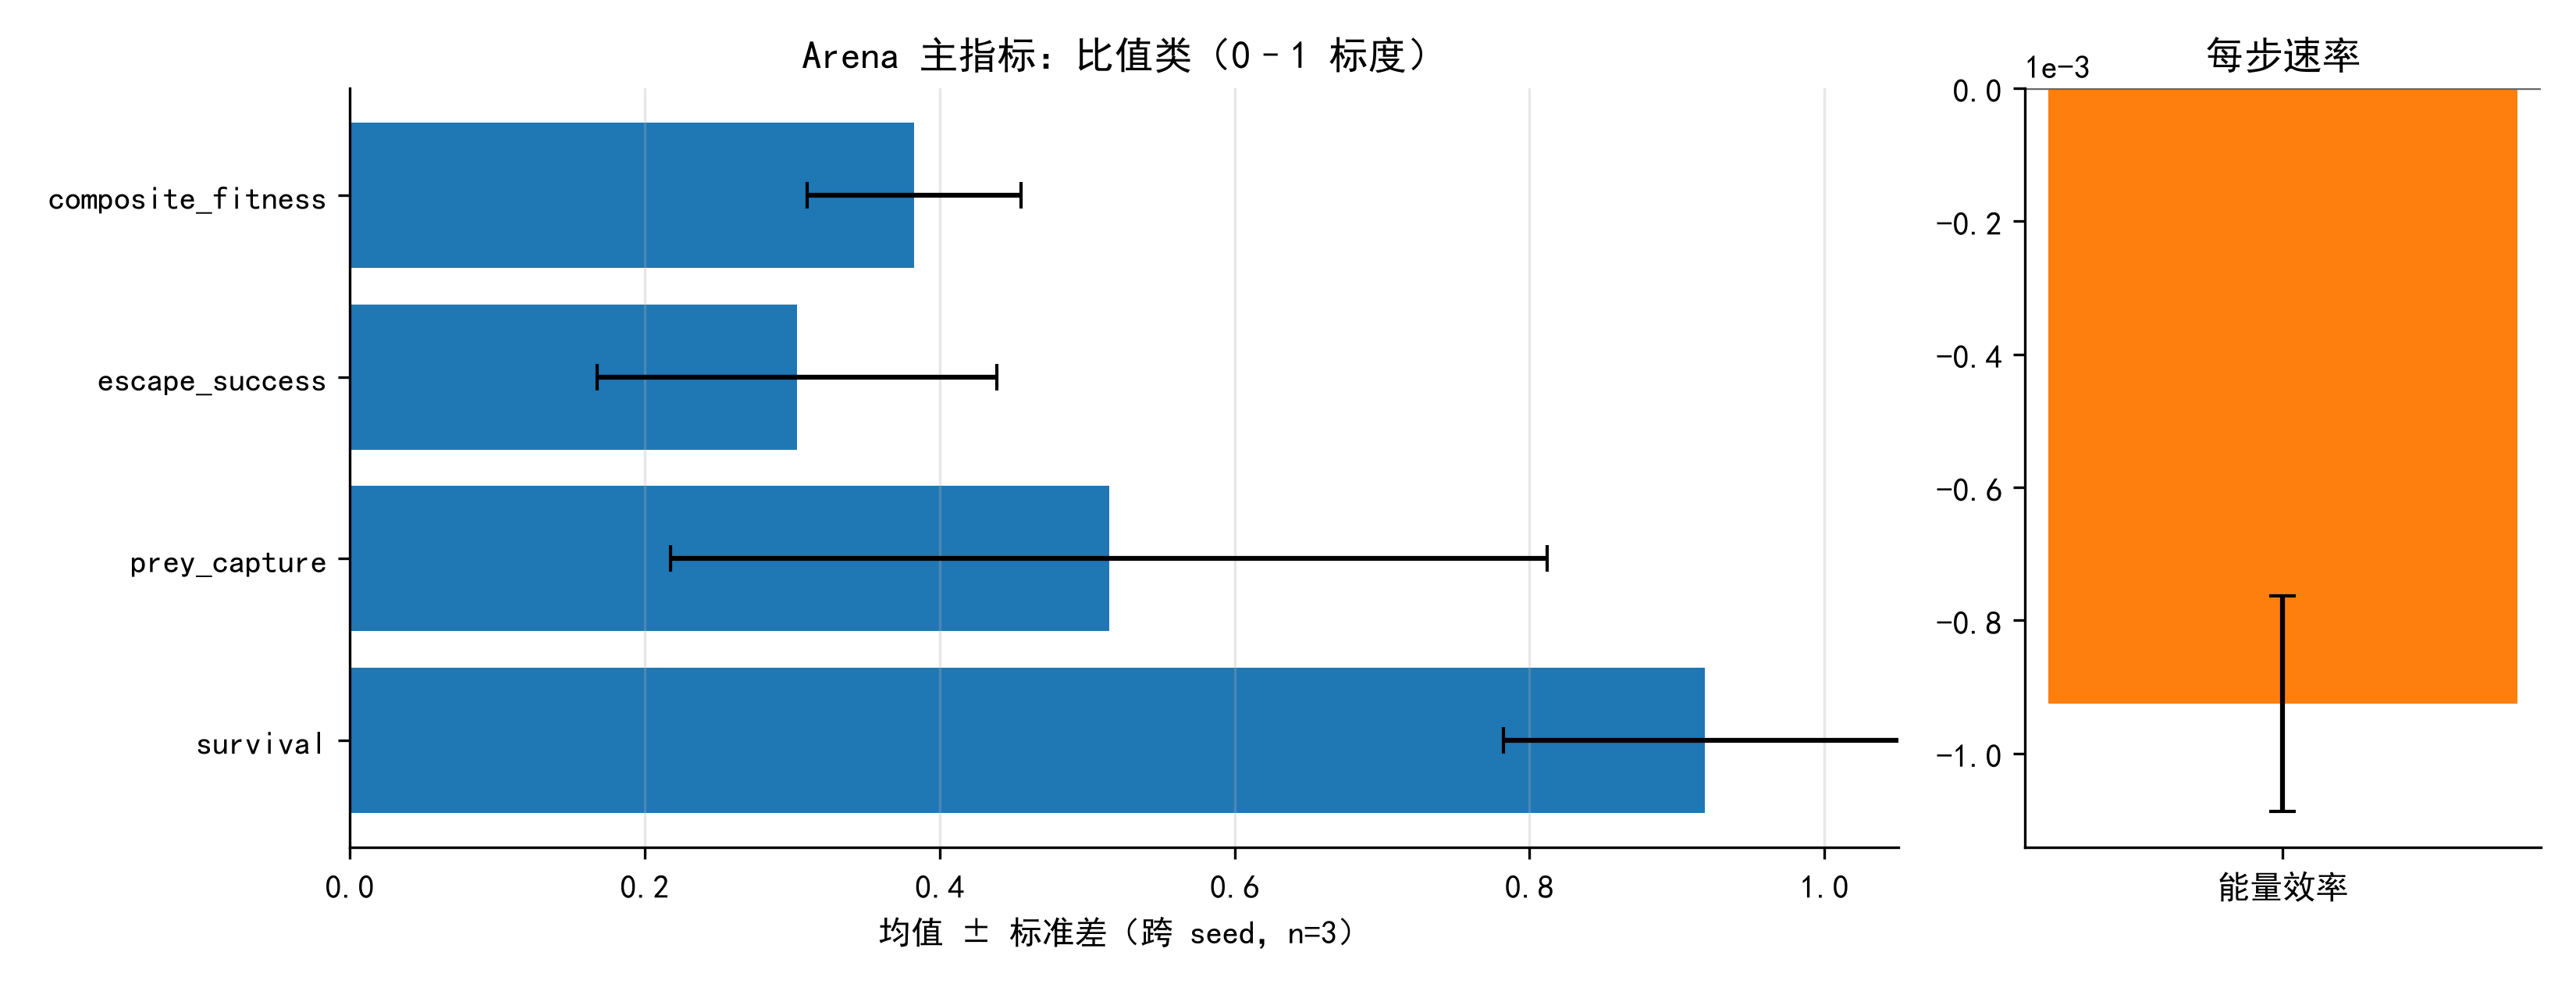
\includegraphics[width=0.95\linewidth]{fig_baseline_v3}
  \caption{ExpertPolicy 冻结基线（3 种子 $\times$ 12 鱼 $\times$ 600 步，跨种子 $\text{mean}\pm\text{std}$）。}
  \label{fig:metrics}
\end{figure}

\subsection{与基线模型的对比（原模型到改后模型）}\label{sec:baselines-ours}

补充说明要求形成「原模型到修改后模型到实验结果对比」。本文以 MLP、GRU、
Fixed Sparse RNN 三类网络为原模型对照，以 DanioNet 为改后模型；
连接数按 $N_{\text{ours}}=151$（支撑边数）反解为 $154$ / $141$ / $154$，
使参数量处于同一数量级（判据 $\left|\Delta\log_{10}\right|\le1$）。
三个评测回合对全部四模型共享同一出生布局与同一条猎物游走，故模型间比较可在块内配对。

表~\ref{tab:expc-models} 给出四模型读数（$2$ 种子 $\times$ $12$ 个体 $\times$ $3$ 回合；
每种子内先对个体与回合等权折叠成一条记录，沿种子轴报 $\text{mean}\pm\text{std}$，$n=2$ 为种子数）。

\begin{table}[H]
  \centering
  \caption{四模型在 Arena 主指标上的读数。}
  \label{tab:expc-models}
  \footnotesize
\setlength{\tabcolsep}{1pt}
  \begin{threeparttable}
  \resizebox{\linewidth}{!}{\begin{tabular}{@{}lcccc@{}}
    \toprule
    指标 & MLP & GRU & Fixed Sparse RNN & DanioNet \\
    \midrule
    \texttt{survival} & $0.9042\pm0.0045$ & $0.9074\pm0.0057$ & $\mathbf{0.9179}\pm0.0322$ & $0.8970\pm0.0075$ \\
    \texttt{capture\_rate} & $0.001042\pm0.000033$ & $0.000903\pm0.000622$ & $\mathbf{0.001111}\pm0.000065$ & $0.000718\pm0.000033$ \\
    \texttt{prey\_capture} & $0.660\pm0.038$ & $0.493\pm0.205$ & $\mathbf{0.677}\pm0.068$ & $0.523\pm0.235$ \\
    \texttt{escape\_success} & $\mathbf{0.3623}\pm0.0246$ & $0.2671\pm0.0707$ & $0.2836\pm0.0409$ & $0.2637\pm0.0560$ \\
    \texttt{energy\_efficiency} ($\times10^{-3}$) & $-1.149\pm0.012$ & $-1.121\pm0.050$ & $\mathbf{-1.114}\pm0.031$ & $-1.159\pm0.111$ \\
    \texttt{composite\_fitness} & $\mathbf{0.3890}\pm0.0065$ & $0.3710\pm0.0120$ & $0.3780\pm0.0194$ & $0.3666\pm0.0085$ \\
    \bottomrule
  \end{tabular}}
  \begin{tablenotes}\footnotesize\raggedright
    \item 数值为 $\text{mean}\pm\text{std}$（沿种子轴，$n=2$，$n$ 为种子数）；加粗为该指标上的最佳基线。
    \item \texttt{prey\_capture} 为个体比值均值口径；\texttt{energy\_efficiency} 为每步非正速率，不与 $0$--$1$ 的比值同轴。
  \end{tablenotes}
  \end{threeparttable}
\end{table}

表~\ref{tab:expc} 给出块内置换检验（块为种子与回合的组合，共 $6$ 个；
同块内四模型共享同一出生布局与猎物游走，故块内置换模型标签在强零假设下精确）。

\begin{table}[H]
  \centering
  \caption{块内置换检验。}
  \label{tab:expc}
  \footnotesize
\setlength{\tabcolsep}{1pt}
  \begin{threeparttable}
  \resizebox{\linewidth}{!}{\begin{tabular}{@{}lccc@{}}
    \toprule
    指标 & $\Delta$（DanioNet $-$ 三基线） & 更高的块 & $p$ \\
    \midrule
    \texttt{survival} & $-0.0128$ & $3/6$ & $0.511$ \\
    \texttt{capture\_rate} & $-0.00030$（$-30\%$） & $2/6$ & $0.076$ \\
    \texttt{prey\_capture} & $-0.0796$ & $2/6$ & $0.459$ \\
    \texttt{escape\_success} & $-0.0407$ & $2/6$ & $0.344$ \\
    \texttt{energy\_efficiency} & $-0.00003$ & $3/6$ & $0.281$ \\
    \texttt{composite\_fitness} & $-0.0127$ & $3/6$ & $0.313$ \\
    \midrule
    \texttt{encounters}（原始计数） & $+7.25$ & $3/6$ & $0.361$ \\
    \texttt{captures}（原始计数） & $-0.181$ & $2/6$ & $0.076$ \\
    \texttt{survival\_steps}（原始计数） & $-7.69$ & $3/6$ & $0.515$ \\
    \bottomrule
  \end{tabular}}
  \begin{tablenotes}\footnotesize\raggedright
    \item 块为种子与回合组合，共 $6$ 个；同块内四模型共享出生布局与猎物游走，块内置换模型标签在强零假设下精确。
    \item $2\times10^{4}$ 次重抽样，$p$ 为蒙特卡洛估计。$\Delta$ 为 DanioNet 减去其余三基线的均值；「更高的块」为 $6$ 块中 DanioNet 领先的块数。
  \end{tablenotes}
  \end{threeparttable}
\end{table}

\emph{读法}：在同等参数量级下，本模型与三类主流网络的\textbf{性能相当}，
差异未达显著（十个受检指标的最小 $p=0.076$），说明三类主流网络已能覆盖本任务的可用性下界。
进一步看，主导读数的是\textbf{评估预算}：块间方差完全淹没模型效应，
\texttt{encounters} 的逐块 $\Delta$ 跨度达 $54.6$，比模型间任何差异大一个数量级，
这也解释了六项主指标为何没有一致排序。由此得到的下一步是先抬高评测回合数，
把模型效应从块间方差里分离出来。$n=2$ 的标准差只有 $1$ 个自由度，
当前结论应读作\textbf{差异未在本轮预算下显现}。

\subsection{环境对照}\label{sec:exp-env-groups}

\textbf{设计原则：单因子对照。}每个环境相对基线只改变一个驱动，
这样观测到的差异才能归因到该驱动。三组环境与基线的取值列于表~\ref{tab:env-groups}；
未被列出的段取默认值。

\begin{table}[H]
  \centering
  \caption{环境对照三组与基线。}
  \label{tab:env-groups}
  \footnotesize
\setlength{\tabcolsep}{1pt}
  \begin{threeparttable}
  \resizebox{\linewidth}{!}{\begin{tabular}{@{}llcccc@{}}
    \toprule
    环境 & 标识 & $n_{\text{prey}}$ & $n_{\text{predators}}$
      & 再生间隔 & 隔离的驱动 \\
    \midrule
    基线 & default & 24 & 3 & 25 & --- \\
    Food Rich & food\_rich & \textbf{48} & 3 & \textbf{13} & 猎物可得性上升 \\
    Predator Rich & predator\_rich & 24 & \textbf{6} & 25 & 捕食压力上升 \\
    Resource Scarce & resource\_scarce & \textbf{12} & 3 & \textbf{50} & 猎物可得性下降 \\
    \bottomrule
  \end{tabular}}
  \begin{tablenotes}\footnotesize\raggedright
    \item 取值属设计选择，无文献实测依据。
  \end{tablenotes}
  \end{threeparttable}
\end{table}

\textbf{派生约定：再生间隔 $=\lceil 600/n_{\text{prey}}\rceil$。}该量随猎物数机械确定，
不是可独立调节的参数。取向上取整：$600/48=12.5$ 恰是平局，
四舍五入会给出 $12$、语义偏向早于名义速率恢复，
而无原则依据；向上取整在平局处无歧义，且统一地取不早于名义速率一侧。

\textbf{前置区分力检查。}在正式跑世代演化之前，先用基线与三环境
$\times$ 3 种子 $\times$ 600 步 $\times$ 12 鱼、以 ExpertPolicy 驱动跑了一轮区分力检查
（表~\ref{tab:env-power}）。表中 $d$ 为环境均值减基线均值再除以合并标准差；$n=3$ 时标准差本身不稳，故 $d$ 仅作指示。

\begin{table}[H]
  \centering
  \caption{环境对照的前置区分力检查。}
  \label{tab:env-power}
  \footnotesize
\setlength{\tabcolsep}{1pt}
  \begin{threeparttable}
  \resizebox{\linewidth}{!}{\begin{tabular}{@{}lcccc@{}}
    \toprule
    指标 & 基线 & \texttt{food\_rich} & \texttt{predator\_rich} & \texttt{resource\_scarce} \\
    \midrule
    survival & 0.9472 & 0.9873 ($d=+1.11$) & 0.8949 ($d=-0.88$) & 0.9464 ($d=-0.02$) \\
    \texttt{prey\_capture}（个体比值均值） & 0.5407 & 0.5324 ($d=-0.08$)
      & \textbf{0.7106} ($d=+1.92$) & 0.5474 ($d=+0.06$) \\
    \texttt{escape\_success} & 0.2292 & 0.2157 ($d=-0.19$)
      & \textbf{0.4491} ($d=+2.89$) & 0.1759 ($d=-1.00$) \\
    \texttt{energy\_efficiency} & $-1.031\text{e-}3$ & $-0.820\text{e-}3$ ($d=+4.12$)
      & $-1.041\text{e-}3$ ($d=-0.30$) & $-1.119\text{e-}3$ ($d=-1.57$) \\
    \texttt{composite\_fitness} & 0.5123 & 0.5216 ($d=+0.24$)
      & \textbf{0.5805} ($d=+1.86$) & 0.5031 ($d=-0.25$) \\
    \midrule
    绝对量：捕获 / 回合 & 55 & \textbf{100} & 55 & \textbf{38} \\
    绝对量：遭遇 / 回合 & 722 & \textbf{2325} & 379 & 323 \\
    \bottomrule
  \end{tabular}}
  \begin{tablenotes}\footnotesize\raggedright
    \item 3 种子 $\times$ 12 鱼 $\times$ 600 步，ExpertPolicy 驱动；括号内为相对基线的效应量 $d$；最后两行为绝对量。
  \end{tablenotes}
  \end{threeparttable}
\end{table}

检查给出三条结论：

\begin{enumerate}
  \item \textbf{\texttt{predator\_rich} 的区分力明确。}\texttt{escape\_success}（$d=+2.89$）、
        \texttt{prey\_capture}（$d=+1.92$）、\texttt{composite\_fitness}（$d=+1.86$）
        三处均超过 $1.9\sigma$，且符号方向符合机制预期（天敌变多，逃逸成功率与接触转化率同时上升）。
  \item \textbf{\texttt{food\_rich} 与 \texttt{resource\_scarce} 的比值指标几乎没有区分力，
        但绝对量差别巨大。}\texttt{food\_rich} 的 \texttt{prey\_capture} $d=-0.08$（几乎为零），
        而捕获绝对数从 $55$ 升到 $100$（$+82\%$）；原因是猎物密度上升同时抬高分子与分母
        （遭遇从 722 升到 2325，$3.2$ 倍），比值把真实效应掩盖了（图~\ref{fig:env-absolute}）。
  \item \textbf{\texttt{food\_rich} 的真实效应落在能量侧。}其 \texttt{energy\_efficiency} $d=+4.12$、
        \texttt{survival} $d=+1.11$，即食物丰富主要通过降低饥饿致死起作用。
\end{enumerate}

\begin{figure}[H]
  \centering
  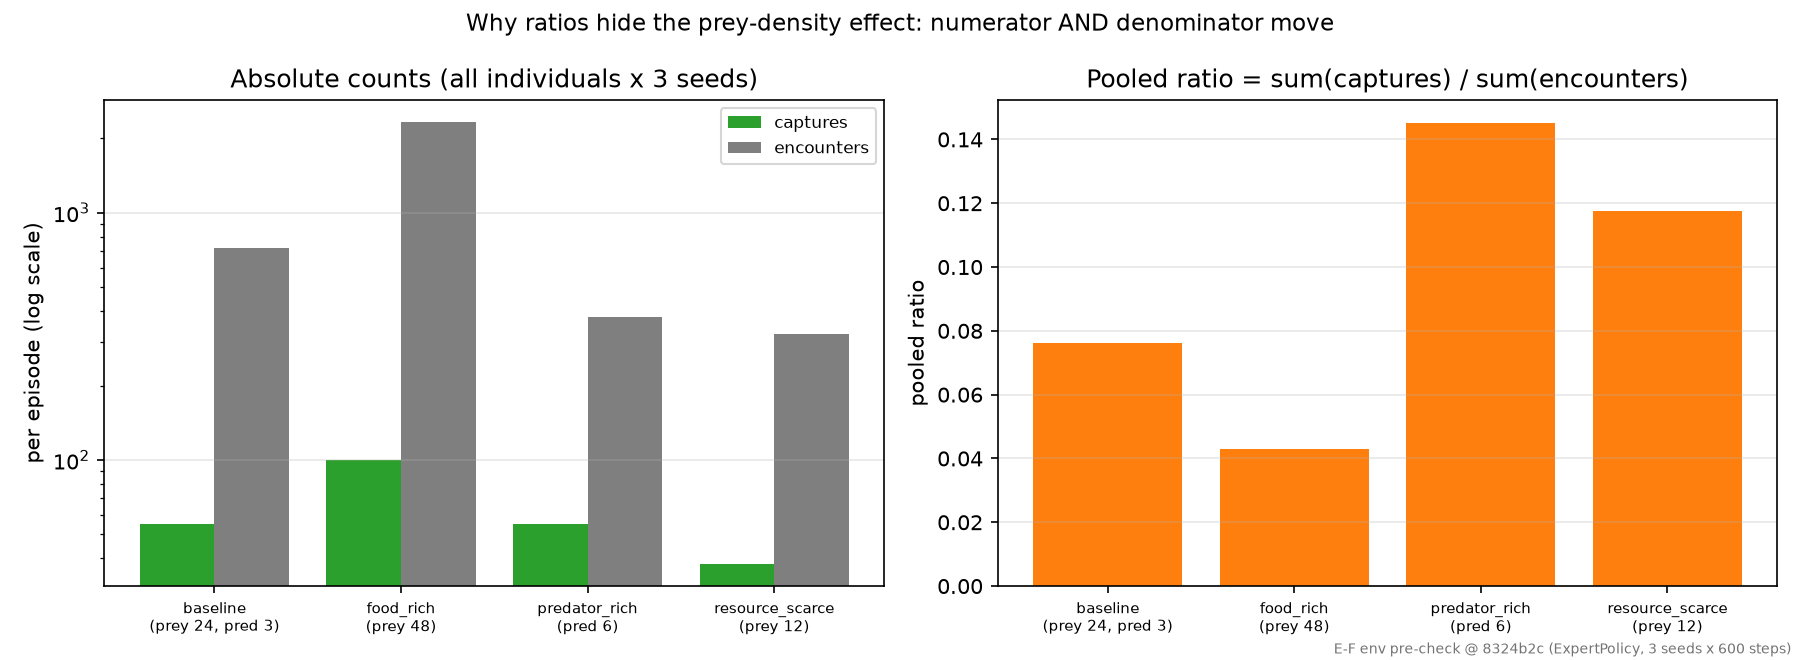
\includegraphics[width=0.95\linewidth]{fig_env_absolute}
  \caption{猎物密度对比值指标的掩盖。}
  \label{fig:env-absolute}
\end{figure}

\subsection{基因型到架构的可辨识性}\label{sec:pen}

发育算子把基因组映射成连接组，但这条映射带有发育期随机性：同一基因型类的个体仍会因随机分裂
落在不同架构档上。以两位点自交的四类基因型为条件，报告观测架构档等于其期望档的比例
$\mathrm{pen}(g)=P(\hat a_i=a^*(g)\mid g_i=g)$。该量是概率性陈述：$\mathrm{pen}<1$
表示基因型只给出架构的偏置，不决定个体命运。

观测轴取神经元数 $N=|M|$。因奠基者背景会使不同随机种子的整体水平平移
（种子间读数中位差约 $8$ 个神经元，而基因型效应约 $1$），$N$ 须\textbf{逐种子居中}
（基线为该种子分层抽样集内读数中位数）后才可跨种子比较；
分裂抽签独立重复 $K=16$ 次取均值，以压低抽样噪声而保留个体发育变异。
校准集与报告集使用不同随机种子，报告集上不再调整阈值。
两种集合的读数与外显率见表~\ref{tab:penetrance}。

\begin{table}[H]
  \centering
  \caption{可辨识性与逐类外显率。}
  \label{tab:penetrance}
  \small
  \begin{threeparttable}
  \begin{tabular}{@{}llll@{}}
    \toprule
    集合 & 分离度 AUC & 最小错分率 & $\theta_N^{\mathrm{obs}}$ \\
    \midrule
    校准集 & $0.8570$ & $0.2219$ & $-0.0312$ \\
    报告集 & $0.8712$ & $0.2158$ & 冻结（取自校准集） \\
    \midrule
    \multicolumn{4}{@{}l@{}}{\emph{报告集逐类外显率（Wilson 95\% 置信区间）}} \\
    \texttt{A\_B\_}（门控期望高） & $0.6975$ & $[0.6709,\,0.7228]$ & \\
    \texttt{A\_bb}（门控期望高） & $0.8892$ & $[0.8701,\,0.9057]$ & \\
    \texttt{aaB\_}（门控期望低） & $0.7908$ & $[0.7669,\,0.8129]$ & \\
    \texttt{aabb}（门控期望低） & $0.7592$ & $[0.7342,\,0.7825]$ & \\
    \bottomrule
  \end{tabular}
  \begin{tablenotes}\footnotesize\raggedright
    \item 校准集 $n=3200$，报告集 $n=4800$（独立样本，阈值取自校准集后冻结）。
  \end{tablenotes}
  \end{threeparttable}
\end{table}

图~\ref{fig:penetrance} 中左为逐类外显率及其 Wilson 区间（虚线为 0.5 机遇水平），
右为两轴分离度 AUC（红虚线为效应量下限 0.70）。

\begin{figure}[H]
  \centering
  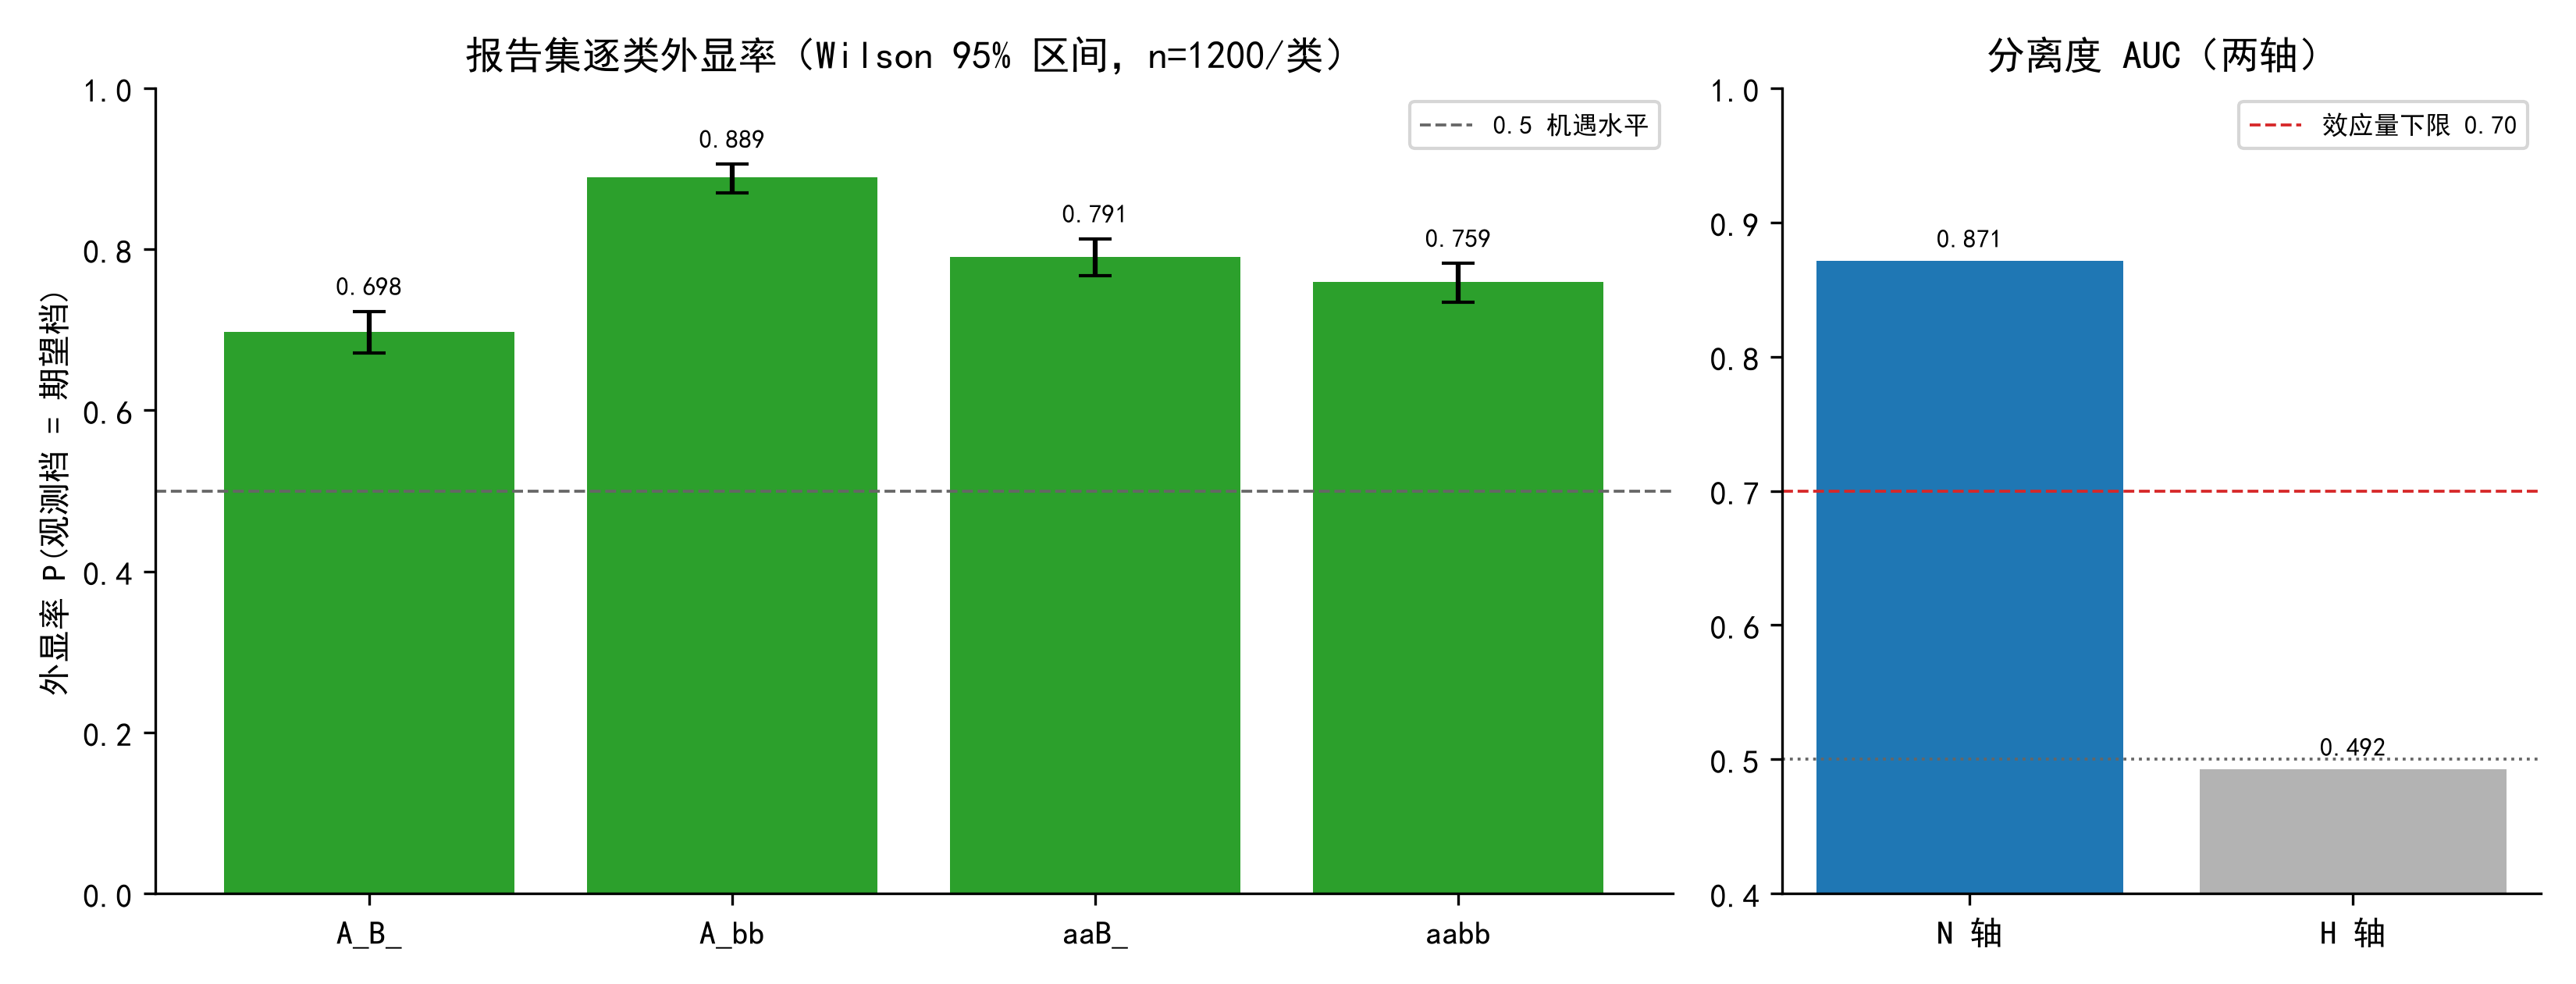
\includegraphics[width=0.98\linewidth]{fig_penetrance}
  \caption{可辨识性报告集（3 种子 $\times$ 4 类 $\times$ 400）。}
  \label{fig:penetrance}
\end{figure}

\noindent\textbf{判据的形式化。}记第 $i$ 个个体的读数为 $N_i$，同种子分层集读数中位数为 $b_s$，
则居中偏差读数为 $\tilde N_i = N_i - b_{s(i)}$。分离度 $\hat\tau_N$ 取
\[
\hat\tau_N \;=\; \frac{1}{n_+ n_-}\sum_{i\in +}\sum_{j\in -}\mathbf{1}\!\left[\tilde N_i > \tilde N_j\right],
\]
即 Mann--Whitney $U$ 统计量除以 $n_+n_-$，对单调变换不变，故不依赖单位规范
（等价于 ROC 曲线下面积，简称 AUC）；
$+$、$-$ 分别为期望档高、低的两类集合。逐类外显率为 $\hat p_g = k_g / n_g$，
区间取 Wilson 得分区间。三点结果：

\begin{itemize}
  \item \textbf{该轴携带基因型信息，且跨种子可迁移。}校准集分离度 $0.8570$，独立报告集 $0.8712$；
        逐种子外显率均未退化到随机水平。
  \item \textbf{外显率不完全。}逐类外显率落在 $0.71$--$0.87$：
        同一基因型类中仍有 $13\%$--$29\%$ 的个体落在另一个架构档，
        故正确读法是\textbf{概率性偏置}，基因型并不决定架构。
  \item \textbf{一根观测轴无区分力。}异质性轴的 AUC 仅 $0.4862$（$p=0.175$，与随机不可分），
        故报告口径取单轴 $N$；异质性轴仍照常测量上报，但不参与判档。
\end{itemize}

\subsection{学习前后对照}\label{sec:bc-results}

学习前后的数值对照尚未取得，本章不含对应结果。

\subsection{典型案例}

本稿未纳入行为轨迹的可视化，逐帧数据可由附录的复现命令重建。
典型案例的动态展示在补充轨迹可视化后给出。

\section{模型检验}\label{sec:validation}

本章从消融、参数敏感性与统计误差三方面检验模型，并说明尚未取得结果的部分。

\subsection{消融实验}

消融用于隔离单个设计变量对结果的影响，设计如下。

\begin{itemize}
  \item \textbf{去掉调控网络（w/o GRN）}：隔离「结构由调控网络发育生成」这一机制；
  \item \textbf{等位基因聚合（加性平均与逐基序取最大）}：隔离显性投影规则；
  \item \textbf{同质时间常数（homogeneous $\tau$）}：隔离异质时间常数的贡献（对应 H3）；
  \item \textbf{去掉空间布线代价（$\lambda=0$）}：隔离空间代价（对应 H4）；
  \item \textbf{行为克隆是否施加 Dale 符号约束}：隔离符号约束；
  \item \textbf{去掉上位效应（w/o epistasis）}：按声明处理。
\end{itemize}

上述消融的完整结果列于后续补充。

\subsection{参数敏感性}

以下参数属设计选择，其取值变动对结论的影响须逐项检验：

\begin{itemize}
  \item 空间布线代价系数 $\lambda$ 与表达相似度系数 $\gamma$：$\gamma$ 取 $\{0.5,1,2\}$ 搜索，
        $\gamma=0$ 作消融；$\lambda$ 有量纲，$\lambda=0$ 作消融，改布局参数必须重定基线。
  \item 适应度四位权重 $(0.35,0.25,0.20,0.20)$：属设计选择，须做敏感性分析。
  \item 突变率 $\mu=0.001$：计算抽象参数，不作生物学解读。
  \item 逐种子居中基线：$N$ 读数跨种子比较前须逐种子居中，否则会得到外显率恒为 $0.5$ 的假象；
        外显率为群体内对比量，不适用于跨批次直接池化。
\end{itemize}

\subsection{统计与误差分析}\label{sec:exp-matrix}

\textbf{分析计划。}表~\ref{tab:analysis-plan} 把五个待检验命题映射到实验与检验口径，不引入新命题。

\begin{table}[H]
  \centering
  \caption{命题、实验与检验口径。}
  \label{tab:analysis-plan}
  \footnotesize
\setlength{\tabcolsep}{3pt}
  \resizebox{\linewidth}{!}{\begin{tabular}{@{}p{0.05\linewidth}p{0.28\linewidth}p{0.17\linewidth}p{0.42\linewidth}@{}}
    \toprule
    命题 & 内容 & 对应实验 & 检验口径（不依赖 $3$ 对 $3$ 置换者标 \checkmark） \\
    \midrule
    H1 & 不同基因组在相同随机种子控制下产生系统性的连接组差异
      & 48 个基因组的完整发育 &
      组内图距离，以重连零模型为基线 \citep{bib20_hartle2020} \checkmark \\
    H2 & 连接组与神经元动力学的差异导致行为差异
      & 发育与行为矩阵 &
      Mantel 检验 \citep{bib21_smouse1986} \checkmark \\
    H3 & 异质 $\tau_i$ 形成与同质 $\tau$ 不同的性能—效率权衡
      & 同质 $\tau$ 消融 &
      性能—效率 Pareto 前沿 \citep{bib23_deb2002} \\
    H4 & 空间布线代价改变网络的局部性、稀疏性与有效边效率
      & 空间代价消融（$\lambda=0$） &
      平均连接距离度量局部性；与图论效率区分命名 \citep{bib22_latora2001} \\
    H5 & $F=F(G,E)$，不存在对所有环境都占优的基因型
      & 同一种群进入三组环境 &
      reaction norm 与 AMMI 检验基因型与环境的秩反转
      \citep{bib24_via1985,bib25_malosetti2013} \\
    \bottomrule
  \end{tabular}}
\end{table}

\textbf{统计能力。}正式实验独立随机种子仅 3 个，$n=3$ 时 $3$ 对 $3$ 标签置换检验的双侧最小
$p\approx0.10$，不足以支持逐命题的置换检验。故 H1 采用组内口径、H2 采用 Mantel 检验，
二者均不依赖 $3$ 对 $3$ 置换；其余结论以效应量与跨种子波动并列报告，
并在结论中显式标注 $n=3$。任何未达显著均不能读作无效应。

\textbf{评估预算与度量饱和（误差来源）。}逐代适应度曲线看不到正向响应，定量归因于两个独立成因：

\begin{itemize}
  \item \textbf{单回合排序几乎不可复现。}把同一个固定种群依次放在 11 个不同的代下标下评估，
        任意两个下标之间个体排序的 Spearman 相关平均仅 $\rho_1=0.069$，
        即选择分数里约 $93\%$ 是代特异噪声。按 Spearman--Brown 校正，
        达到 $\rho\ge0.5$ 需约 14 次平均、$\rho\ge0.7$ 需约 32 次。
  \item \textbf{复合分顶在天花板上。}同一面板中生存分量（权重 $0.35$）有 $81.8\%$ 的观测顶到回合上限，
        复合分中位数恰为该饱和贡献，其余分量达成率仅 $9.7\%$--$13.0\%$。
        即便把测量做到零噪声，选择也只能在一大团并列最高分里挑人，故选择差约等于零。
\end{itemize}

$K$ 次平均同时把并列团分级并把噪声降 $K$ 倍，由此给出可证伪预测：
$K=1$ 时响应约等于零，$K\approx14$ 时应出现正向响应。该预测由后续的多回合代循环实验检验。

\subsection{已知局限}\label{sec:exp-gaps}

以下各项是当前尚未闭合的度量或结果：

\begin{itemize}
  \item 捕获默认确定性（满足几何条件即必定捕获），使一部分指标偏乐观：
        实测进过口但吃不下的判定为零，捕食技巧这一维度几乎未被检验。
        启用非确定性捕获后，失败会记为未命中，接触转化率自动成为真成功率。
  \item 学习前后对照、完整消融、多代演化正式结果与效率三项（时延、浮点运算量、峰值内存）
        均尚未取得落盘结果。
  \item 观测编码的取值规则属设计选择，其与像素输入的差异是本文的建模假设之一。
\end{itemize}

\section{模型评价与推广}\label{sec:evaluation}\label{sec:limitations}

\subsection{模型优点}

本文的贡献是把一组互相约束的问题做成了可重跑、可反驳的计算实验。
机制内核是一对组合：网络架构由可演化的生成式编码产生，学习被限制为冻结结构上的当代权重扰动、
且不接受其遗传。由此带来四点价值：

\begin{enumerate}
  \item \textbf{把可搜索的对象上移了一层。}被搜索的是生成结构的基因组，
        于是两类结构变异来源同时变得可测量：同源基因组与不同随机种子、单碱基扰动，
        分别对应 H1 与 H2。代价是支撑与符号在训练期冻结，当代无法改变结构。
  \item \textbf{「后天不遗传」由一句引言变为可测量的对照。}结构冻结、只训当代权重，
        于是当代可塑性带来多少与发育结构本身承担多少在机制上被分开，可分别测量。
        若当代扰动显著改善行为而结构完全不变，则当代可塑性足以承担任务；反之则负担主要在发育结构。
  \item \textbf{可用与多样在同一条链上度量。}可用性走闭环生态仿真，多样性走组内图距离与 Mantel 检验；
        这两个判据不依赖跨种子显著性，故在仅有 3 个正式种子的预算下依然可给出结论。
  \item \textbf{输出同源，使结论可被他人复核。}整条生成链确定性推进，
        事件日志、实验指标与专家轨迹三条输出共用同一编号，故每个报告数字都能回溯到运行产物。
\end{enumerate}

\subsection{适用边界}

\begin{enumerate}
  \item \textbf{规模与外推。}实测结构规模为神经元数中位 $37.0$（$27$--$43$，上限 $48$）、
        支撑连接中位 $192.5$ 条（$105$--$289$），比主流任务上 $10^{6}$--$10^{9}$ 参数的网络小若干数量级。
        本平台回答某机制是否存在、幅度多大；该机制在大规模任务上是否仍有效，超出其外推范围。
  \item \textbf{度量与场景。}默认配置下捕获是确定性的，捕食技巧维度未被检验；
        六类细胞类型是功能抽象，结构统计的结论不直接映射到真实细胞类型计数；
        评价场景限于连续二维觅食—避敌。度量上，三个都叫捕获率的量相差约 7 倍、
        分母严重右偏、能量效率为每步非正速率，引用均值时须并列偏态尾与绝对量。
  \item \textbf{统计预算。}正式种子为 3，$n=3$ 时 $3$ 对 $3$ 置换检验双侧最小 $p\approx0.10$，
        跨条件比较以效应量与跨种子波动为准。环境三组中 \texttt{predator\_rich} 区分力明确，
        另两组只有绝对量差别明显（捕获由 $55$ 增至 $100$，或降至 $38$）。
  \item \textbf{训练链的完成度。}演化与学习的联合效果尚未验证；
        学习前后对照、完整消融与多代正式结果正在按计算预算推进。
        外显率也不完全（$0.71$--$0.87$），基因型给出的是架构的概率性偏置。
\end{enumerate}

\subsection{改进方向}

优先级由误差分析给出：先抬高评测回合数（近免费），把模型效应从块间方差里拉出来；
再启用非确定性捕获，使捕食技巧成为可检验维度；随后补齐行为克隆接入与消融、
落盘多代演化正式结果、补出时延与计算量等效率指标。上述任一改进都须重新声明基线口径。

\subsection{推广价值}

本文的可迁移之处有三。其一，闭环生态仿真把「可用与多样」放在同一条链上度量，
该框架可迁移到其他感知—动作耦合的序贯决策任务。其二，把可演化对象上移到基因组、
以发育算子生成结构，为神经演化的生成式路线提供了一条可复现的实验路径。
其三，确定性重放与同源输出使结论可被第三方复核，适合作为教学与可视化平台。

\section{AI 使用声明}\label{sec:ai-decl}

本节说明生成式 AI 在本项目中的使用范围、边界与责任归属，依据是赛题允许使用 AI
但须体现参赛者的设计判断，以及评分标准对 AI 使用声明严谨程度的考察要求。

\subsection{使用范围}

生成式 AI 在本项目中承担辅助性工作：资料检索线索整理、建模方案讨论、代码草拟与调试、
测试用例设计、文字整理、可视化方案构思，以及装饰性视觉素材的生成。

\subsection{边界}

\begin{itemize}
  \item \textbf{不生成实验数据}：本文的实验数据、模型指标、统计图与网络结构图
        均由实际程序运行产生。AI 生成的装饰性图像不作为实验数据或科学证据。
  \item \textbf{不填未定数值}：上游文档未定义的数值、公式与语义，实现侧不得自行选定并当作既定事实。
        本文引用的每个数字均可回溯到运行产物或配置；未跑完的实验留空并注明，不以估算替代。
  \item \textbf{不替代核心设计}：问题定义、数学模型（发育映射、网络动力学、遗传边界与当代学习）、
        实验设计与结论判断均由团队成员完成，AI 仅作为实现与整理的加速工具。
\end{itemize}

\subsection{责任归属}

团队成员对问题定义、数学模型、代码、数据、实验、统计分析、文献引用、
技术报告与最终路演陈述进行人工审核，并承担最终责任。


\appendix
\section{复现说明}\label{sec:repro}

\subsection{环境与依赖}

后端与实验以 \texttt{uv} 管理环境，并以\textbf{锁文件}安装（\texttt{uv sync --frozen}），
项目要求 Python $3.12$ 及以上。论文用 \texttt{xelatex}（\texttt{ctex} 的中文排版依赖它）编译，
中文草稿的编译命令为 \texttt{latexmk -xelatex main.tex}。

\subsection{从随机种子到运行产物}

\textbf{子种子派生。}所有随机过程由 master seed 经 NumPy \texttt{SeedSequence} 统一派生：
命名空间序号取列表熵 $S_{ns}=\texttt{SeedSequence}([ns,\ master\_seed])$，
实体序号 $t$ 取 $S_{ns}.\texttt{spawn}(k)[t]$，整数子种子由
$C.\texttt{generate\_state}(1,\texttt{uint32})[0]$ 给出。两条约束直接决定换台机器能否对上：
变化 ID 前置（取 $[ns, master\_seed]$），
且实体序号必须由稳定标识确定性映射，不得使用调用顺序。

\textbf{正式种子与运行目录。}正式实验固定种子 $[1103,2207,3301]$；
演示种子单独固定，与实验种子隔离。每个种子对应一个独立运行目录，
逐个体原值全部留在该目录，任何人都可据此重算汇总数，不必信任正文报出的汇总值。

\subsection{全流程命令链}

以下脚本按顺序执行即得本文全部数字；除第一个外都只读上游产物，可重复执行而不改变语义。

\begin{itemize}
  \item \texttt{run\_experiment.py --config <cfg> --seed <s> --experiment-id <id>}：
        建立运行目录并固定配置快照、种子与代码版本，是目录布局的唯一来源；
        同一 \texttt{(id, seed)} 只能建一次，已存在即报错退出。
  \item \texttt{run\_arena.py --experiment-id <id> [--seeds 1103,2207,3301]}：
        跑 $20$\,Hz $\times$ $600$ 步每回合，落逐个体指标、逐回合事件计数、
        事件日志与逐种子汇总，并写出跨种子 $\text{mean}\pm\text{std}$。
  \item \texttt{make\_figs.py --experiment-id <id>}：
        只读运行目录，出逐种子诊断图与跨种子报告图，并为每张图导出同名数据表。
  \item \texttt{make\_tables.py --experiment-id <id>}：
        出汇总表、口径诊断、逐个体明细与逐回合明细。
  \item \texttt{run\_penetrance.py --experiment-id <id> --mode calibrate|report}：
        出可辨识性的校准与报告产物（两口径、轴向分离度、逐类置信区间）。
\end{itemize}

\subsection{图与数据的对应}

每张跨种子报告图都带\textbf{来源脚注}（运行标识与代码版本），拿到一张图即可回到产生它的那次运行。
图的文字一律用英文，中文叙述放表格。每张图都有同名数据表：约定为
\texttt{<图目录>/<图名>.png} 配 \texttt{<图目录>/data/<图名>.xlsx}，同名即对应；
每个工作簿的第一张表固定为清单，逐表写明来源、口径与溯源项，其余表为原始数据。
这样后续统一美化时可以改样式而不改数据，也便于第三方直接取数复算。

\subsection{确定性与最脆弱处}

生态仿真侧的确定性由两条机制保障：每次重置会重建随机源，故同一环境反复重置得到逐字段一致的初始局面；
每步的随机数消费只由该步状态决定，故推进到第 $k$ 步与分几次调用推进到第 $k$ 步无关。
最脆弱的一环是出生布局的拒绝采样：其采样次数取决于当前障碍布局，
故改动障碍数量、半径范围或间距会使后续所有实体的随机流整体平移，同一随机种子下的初始世界随之改变，
历史基线不可直接对比。种子固定的只是随机流；语义一改，同种子的两局即不再属于同一实验。
环境对照遵守单因子原则，未被列出的段一律取默认值。


\bibliographystyle{gbt7714-numerical}
\bibliography{refs}

\end{document}
